\chapter{Simulaci\'on y caracterizaci\'on de la emisi\'on de radio en eventos ES}
\label{ch:simulacionRadio}

Tal como se describi\'o en el cap\'itulo \ref{ch:easRadio}, la emisi\'on de radio de las lluvias atmosf\'ericas extendidas conforman un fen\'omeno complicado, por lo que su c\'alculo se aborda usualmente mediante modelos macrosc\'opicos efectivos o a trav\'es de una representaci\'on microsc\'opica ligada al uso de t\'ecnicas de Monte Carlo.
En esta tesis se opt\'o por el segundo tratamiento por dos razones; la primera consiste en que hasta el momento no hay modelos efectivos desarrollados para lluvias ES y la segunda es que este enfoque permiti\'o utilizar la experiencia adquirida al calcular la exposici\'on de Auger en esta nueva tarea.

En la primer parte de este cap\'itulo se describe la cadena de simulaciones utilizada para calcular la se\~nal esperada sobre un arreglo de antenas de radio al detectar neutrinos ES, necesarias para realizar el c\'alculo de exposici\'on.
En particular, se exponen las caracter\'isticas m\'as relevantes del algoritmo de c\'alculo de la se\~nal utilizado por \zhs{}, la extensi\'on de \aires{} que incluye la simulaci\'on de la emisi\'on de radio de las EAS.

En la segunda parte se realiza una caracterizaci\'on de la huella de campo el\'ectrico dejada por lluvias atmosf\'ericas iniciadas por neutrinos ES.
\textbf{COMPLETAR}

\section{Simulaci\'on de la se\~nal}
\label{sc:simRadio}
	
	Como se discuti\'o en el cap\'itulo \ref{ch:simulacionAuger}, la simulaci\'on de eventos ES requiere tres etapas: la simulaci\'on de la interacci\'on primaria, el desarrollo de la lluvia atmosfrica y el c\'omputo de la se\~nal sobre el detector.
	A la hora de simular la emisi\'on de radio se requieren las mismas etapas:
	%
	\begin{description}
		\item[Interacción primaria:] Al igual que en la primer parte de esta tesis, la interacci\'on neutrino nucleon se proces\'o utilizando \tauola{}, que fue descripto en la secci\'on \ref{sbsc:tauola}.
		\item[Desarrollo de la EAS:] como se discuti\'o en la secci\'on \ref{sc:gen_emision} a nivel microsc\'opico la emisi\'on de radio de una EAS puede conseguirse como superponiendo las de cada part\'icula de la lluvia. bajo este principio, el programa \zhs{}, una modificaci\'on de \aires{}, implementa la aproximaci\'on ZHS (ver secci\'on \ref{sbsc:zhs_approx}) sobre cada una de las part\'iculas simuladas. La descripci\'on de \zhs{} se realiza en la secci\'on \ref{sbsc:zhaires}.
		\item[Señal en el detector:] La salida de \zhs{} consiste en el campo el\'ectrico en funci\'on del tiempo sobre una lista de observadores (antenas) ubicados en posici\'ones puntuales del espacio. Para transformar esta se\~nal \emph{cruda} en la obtenida por una antena real es necesario aplicar una serie de algoritmos, que se describen en la secci\'on \ref{sbsc:sig_treat}.
	\end{description}
	
	\subsection{ZHAireS}
	\label{sbsc:zhaires}

	\zhs{} es una implementaci\'on del las rutinas de ZHS \cite{1_halzen_zas_stanev_1991,2_zas_halzen_stanev_1992} sobre \aires{} desarrollada por Jaime Alvarez-Muñiz, Washington Rodriguez-Carvhalo Jr. y Matias Tueros en el Departamento de Física de Partículas Universidad de Santiago de Compostela, España.
	\zhs{}, conserva todas las capacidades de \aires{} y agrega la posibilidad de simular el la emisi\'on de radio de la EAS, incluyendo nuevas directivas de entrada que permiten controlar con buen detalle la simulación.
	
		\subsubsection{C\'omputo de la se\~nal}
		
		La metodolog\'ia aplicada en \zhs{} para calcular la se\~nal es simple: cada vez que el algoritmo de \aires{} avanza una part\'icula se llama a las rutinas de ZHS, una implementaci\'on en fortran de las aproximaciones ZHS.

		Como se mencion\'o en la secci\'on \ref{sbsc:zhs_approx}, para que las aproximaciones sean v\'alidas, es necesario cumplir las siguientes hip\'otesis:
		\begin{enumerate}
		\item La inversa distancia entre cualquier punto del track y el observador debe poder ser considerada una constante.
		\item La longitud del track es peque\~na a comparaci\'on de la distancia al observador.
		\item El observador se encuentra en la zona de campo lejano.
		\end{enumerate}
		%
		Por ende, si el tama\~no de los tracks obtenidos a partir del algoritmo de \aires{} no siatisface alguna de las condiciones 1 o 2, una rutina se encarga de partirlo en trozos lo suficientemente chicos como para que suceda.
		Por otro lado, si no se llegara a cumplir la condici\'on n\'umero 3, ser\'ia necesario utilizar la soluci\'on exacta del problema, lo que no se encuentra implementado en \zhs{} hasta el momento.
		Esta es una limitaci\'on conocida del c\'odigo, que genera se\~nales artificiales cuando las part\'iculas propagadas se encuentran muy cerca de las antenas.
		Afortunadamente, la contribuci\'on de estas part\'iculas es poco importante incluso en EAS que se desarrollan muy cerca del detector como las iniciadas por neutrinos ES, debido a que la mayor parte de la se\~nal proviene de regiones cercanas al eje de la lluvia.
		
		Una vez que los tracks cumplen las condiciones necesarias el campo el\'ectrico se calcula mediante la ecuaci\'on \ref{eq:efield_0}, descripta en la secci\'on \ref{sbsc:zhs_approx}.
		
% 		, se calcula el potencial vector $\vec{A}(t,\hat{u})$ y el campo el\'ectrico $\vec{E}(t,\hat{u})$ en la posici\'on del observador utilizando las ecuaciones \ref{eq:afield} y \ref{eq:efield}.
% 		\begin{equation}
% 		\vec{A}(t,\hat{u})
% 		=
% 		\frac{\mu e}{4\pi Rc}
% 		\vec\beta_{\bot}
% 		\frac{\Theta(t-t^{det}_1)-\Theta(t-t^{det}_2)}{1-n\vec\beta\cdot\hat u}
% 		\label{eq:afield}
% 		\end{equation}
% 	% 	$\vec E(t)=-\partial\vec{A}/\partial t $
% 		\begin{equation}
% 		\vec{E}(t,\hat{u})
% 		=
% 		-\frac{\mu e}{4\pi Rc}
% 		\vec\beta_{\bot}
% 		\frac{\delta(t-t^{det}_1)-\delta(t-t^{det}_2)}{1-n\vec\beta\cdot\hat u}
% 		\label{eq:efield}
% 		\end{equation}
% 		En estas, como en la figura \ref{fig:trackSch}, $\hat{u}$ es el versor que indica la direcci\'on entre la mitad del track y el observador, $\vec\beta=\vec v/c$, $\vec\beta_{\bot}=-[\hat{u}\times(\hat{u}\times\vec\beta)]$ es la proyecci\'on de $\vec\beta$ sobre el plano perpendicular a $\hat u$ y $t_{1,2}^{det}=t_{1,2}+nR/c-n\vec\beta \cdot \hat u (t_{1,2}-t_0)$ son los tiempos de detecci\'on del principio y final del track respectivamente, con $t_0=(t_1+t_2)/2$. Por otro lado, $\Theta(x)$ y $\delta(x)$ son las funciones escalón de Heaviside y delta de Dirac respectivamente.
		
		Por otro aldo, para calcular correctamente el tiempo de arrivo de la se\~nal a la antena, es necesario tener un modelo que describa el \'indice de refracci\'on de la atm\'osfera.
		Dado que el camino \'optico puede ser escrito como una integral de linea, dada una trayectoria, y haciendo uso del teorema del valor medio integral, se puede definir un \'indice de refracci\'on efectivo seg\'un:
		%
		\begin{equation}
			\begin{matrix}
			n_{eff}
			=
			1+{\mathcal R}_{eff}\times10^{-6}
			&
			{\rm con}
			&
			{\mathcal R}_{eff}
			=
			\frac{1}{R}\int_0^R{\mathcal R}(h)dl
			\end{matrix}
		\label{eq:refIndexEff}
		\end{equation}
		%
		donde, ${\mathcal R}(h) = \left[ n(h)-1 \right] \times 10^6$.
		Para ${\mathcal R}(h)$, \zhs{} ofrece la posibilidad de utilizar un valor constante, o un modelo exponencial como el de la ecuaci\'on \ref{eq:refIndexExp}, en el que es posible fijar su valor a nivel del suelo.
		\begin{equation}
		{\mathcal R}(h)
		=
		{\mathcal R}_o
		\exp{-K_rh}
		\label{eq:refIndexExp}
		\end{equation}
		Los valores por default son ${\mathcal R}_o={\mathcal R}(h=0)\equiv 325$ y $K_r=0.1218km^{-1}$.
		Con estos valores es posible reproducir los valores calculados en \cite{gerson1948polar} con un $1\%$ precisi\'on hasta una altura de \cant{20}{km}.
		A mayor altitud la aproximaci\'on exponencial para ${\mathcal R}$ sobreestima el \'indice de refracci\'on, pero m\'as all\'a de los \cant{20}{km} la lluvia recien ha comenzado a desarrollarse, por lo que la cantidad de part\'iculas es relativamente peque\~na por lo que esta zona contribuye muy poco a la se\~nal total.
		
		En esta tesis se utiliz\'o el modelo exponencial para el \'indice de refracci\'on con ${\mathcal R}_o=325$ y $K_r=0.1218km^{-1}$ en todas las simulaciones.
		
		Otro factor a tener en cuenta aparece cuando las lluvia a simular es muy inclinada.
		Dado que la cascada puede iniciarse a cientos de kilometros del detector, la aproximaci\'on de tierra plana no es v\'alida.
		Por ende, la altura que se utiliza en la ecuaci\'on \ref{eq:refIndexExp} debe ser medida cuidadosamente, incluyendo la curvatura de la tierra, como se muestra en la figura \ref{fig:refIndex}.
		%
		\begin{figure}[ht!]
		\centering
			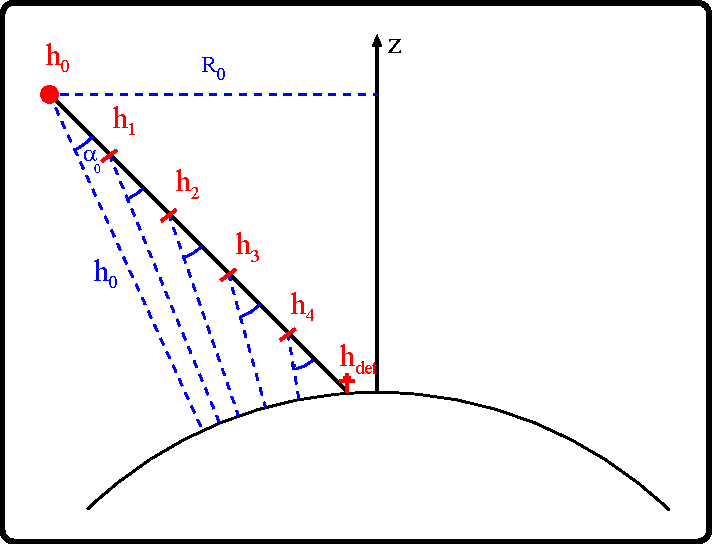
\includegraphics[width=0.6\textwidth]{fig/simulacionRadio/refIndex}
			\caption{\label{fig:refIndex} Esquema del m\'etodo mediante el que se tiene en cuenta la curvatura de la tierra al momento de calcular el \'indice de refracci\'on de la atm\'osfera para diferentes alturas.}
		\end{figure}
		%
		Dado que realizar la integral descripta en \ref{eq:refIndexEff} en estas condiciones resulta computacionalmente muy costoso, en \zhs{} se discretiza la distancia $R$ en un n\'umero finito de tramos y supone el \'indice de refracci\'on constrante en cada uno de ellos.
		
		Una vez calculadas las amplitudes de los campos y los tiempos de arrivo de las se\~nales debidas a cada track, el campo total en cada observador se guarda utilizando bines temporales prefijados, como la ecuaci\'on \ref{eq:eAntField}, donde el \'indice $j$ recorre las part\'iculas simuladas y $\omega_j$ representa el peso estad\'istico de la part\'icula\footnote{Este peso es el peso asignado por el algoritmo de thinning durante la simulaci\'on.} que emiti\'o el campo $\vec{E}_j$.
		\begin{equation}
		\vec{E}(t_i)=\sum_{j:t_j\varepsilon[t_i,t_{i+1}]}\vec{E}_j(t_j)\omega_j
		\label{eq:eAntField}
		\end{equation}
		%
		De la ecuaci\'on \ref{eq:eAntField} es posible notar que la se\~nal simulada en una dada antena depende fuertemente del algoritmo de thinning utilizado. 
		Dado que la mayor contribuci\'on al campo el\'ectrico proviene de las part\'iculas de media y baja energ\'ia, es poco deseable la aparici\'on de partículas con peso extremadamente alto.
		En consecuencia y como bajar el nivel de thinning es poco eficiente, en la simulación se utiliza un \emph{weight factor} peque\~no.
		
		
		\subsubsection{Dificultades técnicas}

		Con el fin de no volver tediosa esta sección a continuaci\'on se enumeran una serie de dificultades técnicas presentes a la hora de simular la señal de radio emitida por neutrinos ES utilizando \zhs{}.

		En primer lugar, al igual que en las simulaciones realizadas con \aires{} para calcular la exposici\'on de Auger, es necesario utilizar los productos de decaimiento del \tauon{} generados con \tauola{} como condici\'on inicial en \aires{}.
		La dificultad en este paso subyace simplemente en conciliar los sistemas de coordenadas en los que se describen las posiciones y velocidades en \tauola{} y \aires{}.

		Luego, la mayor dificultad técnica resulta de la gran cantidad de tiempo de máquina que requiere realizar la simulación de la emisión de radio.
		Para contextualizar la situación, una simulación típica puede implicar el c\'alculo de la señal en algunos cientos de observadores.
		Dado que cada vez que se avanza una partícula es necesario calcular la señal en cada uno de ellos, luego de la primer decena de antenas el tiempo de simulación depende casi linealmente de su numero, es decir, el tiempo que toma simular la evolución de la lluvia se torna despreciable.
		Con todo esto, como la simulación de una lluvia de \cant{10^{18}}{eV} puede tomar del orden de algunas horas por decena de anteas\footnote{Este número depende fuertemente del nivel de thinning elegido}, la simulación completa de cada lluvia puede requerir del orden del centenar de horas de tiempo de CPU.
		La única manera de salvar este inconveniente es partiendo el detector en grupos mas pequeños de antenas, de entre 10 y 40, donde es necesario tener la precaución de que la evolución de la lluvia se simule con la misma semilla en cada vez.
		Una vez finalizada cada simulaci\'on se utilizaron una serie de programas en c++ para compaginar los eventos y luego analizarlos.
		
		\subsubsection{Desempe\~no de \zhs{}}
		
		Finalmente, es necesario hacer menci\'on del desempe\~no alcanzado por \zhs{} para describir la se\~nal generada por lluvias atmosf\'ericas ya que los resultados de esta parte de la tesis depender\'an fuertemente del mismo.
		En la figura \ref{fig:zhsvsdata}, tomada de \cite{cite:icrc13Auger}, se compara la distribuci\'on lateral\footnote{La distribuci\'on lateral en este caso se refiere a la dependencia de la amplitud m\'axima observada en la antena con la distancia radial respecto del centro de la lluvia.} de un evento de AERA, la extensi\'on de radio del proyecto Pierre Auger, con la obtenida mediante \zhs{}.
		%
		\begin{figure}[ht!]
		\centering
			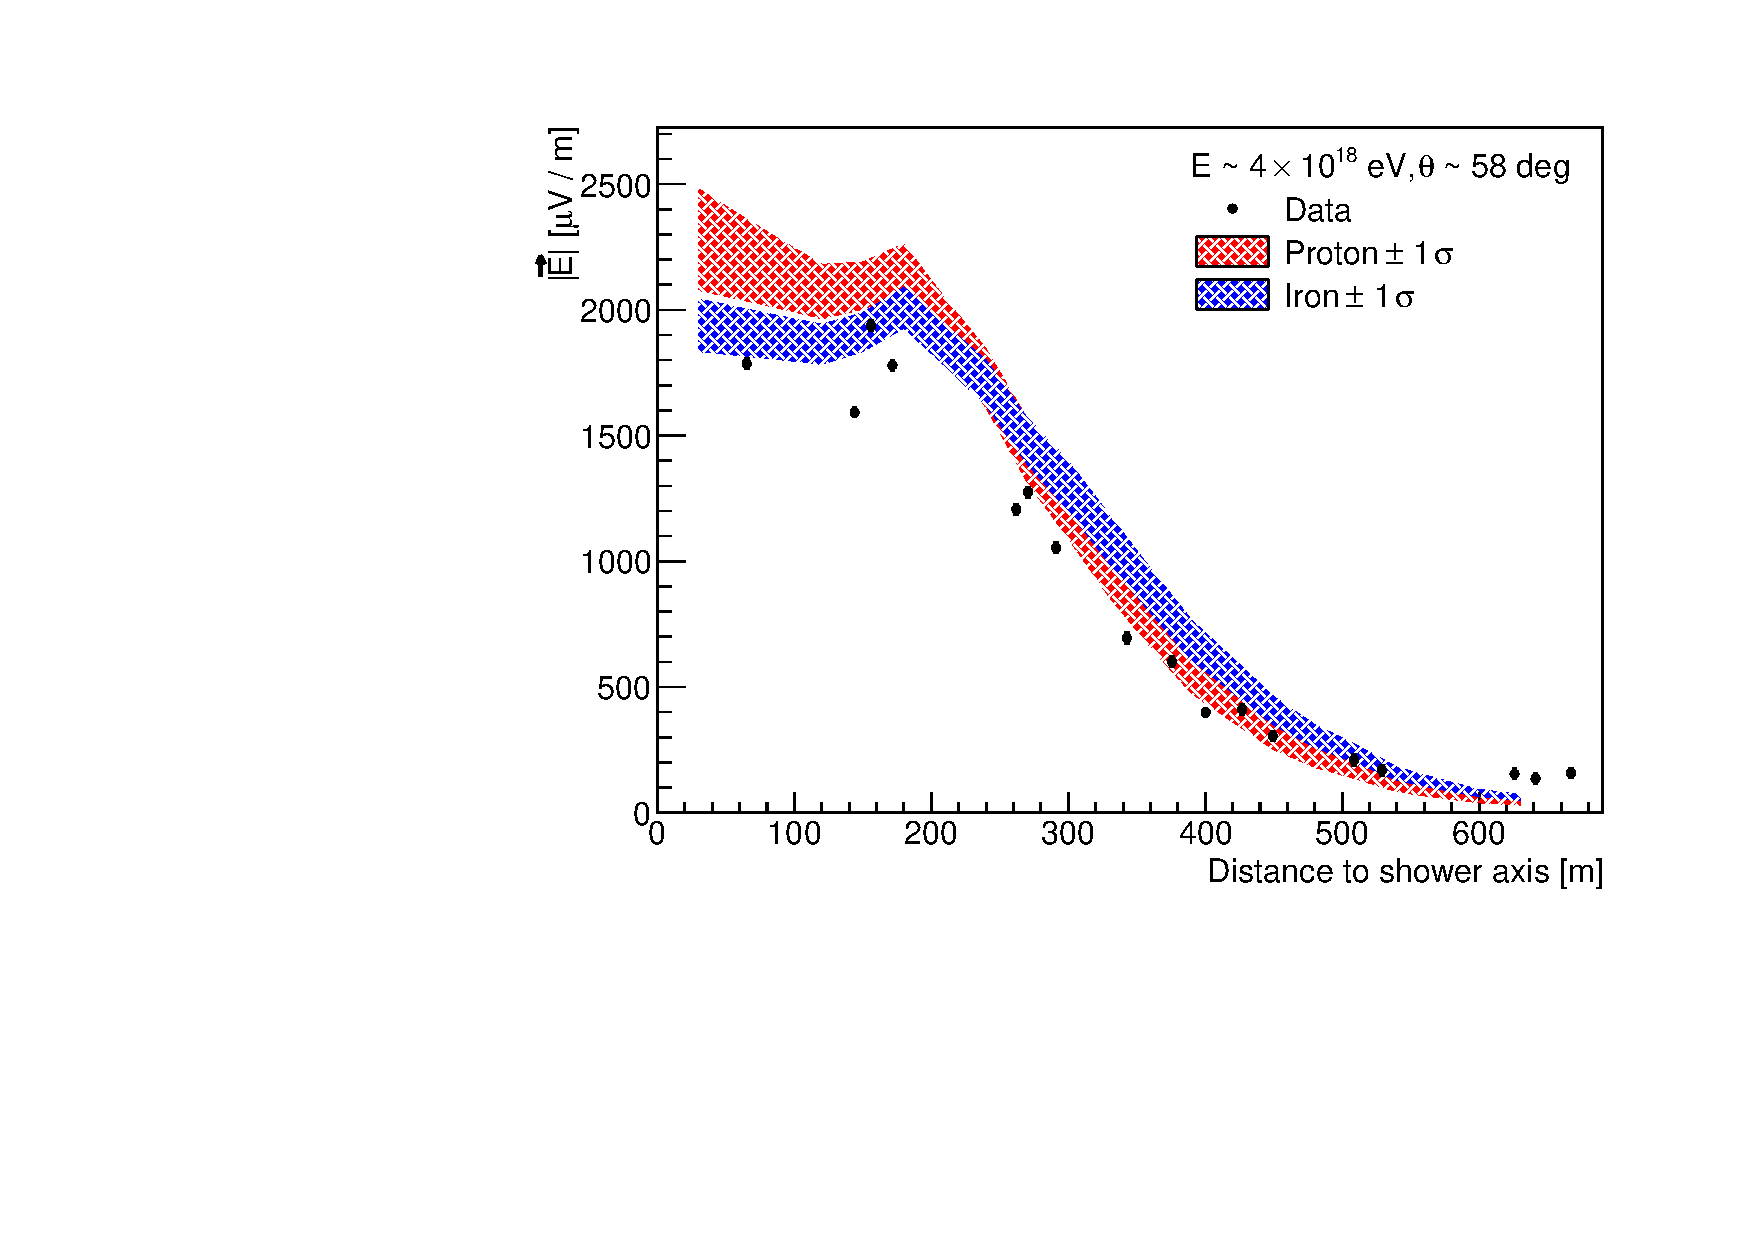
\includegraphics[width=0.6\textwidth]{fig/simulacionRadio/ZHAireS_and_data}
			\caption{\label{fig:zhsvsdata} Tomada de \cite{cite:icrc13Auger}. Comparaci\'on entre la distribuci\'on lateral de un evento de AERA y la obtenida utilizando \zhs{}. Los par\'ametros utilizados para la simulaci\'on se obtuvieron de la reconstrucci\'on del evento. La franja roja representa la zona $\pm1\sigma$ para protones mientras que la azul para eventos iniciados por hierro.}
		\end{figure}
		%
		Como par\'ametros de entrada de las simulaciones se utilizaron los obtenidos en la reconstrucci\'on realizada con el detector de superficie del observatorio. 
		Debido a la falta de informaci\'on sobre el primario de la lluvia, se realizaron simulaciones utilizando protones y hierro. La franja roja representa la zona $\pm1\sigma$ para protones mientras que la azul para eventos iniciados por hierro.
		Este resultado muestra un grado de acuerdo dentro del $10\%$ en esta variable (la amplitud de la se\~nal).
		
		M\'as adelante, se utilizar\'a la distribuci\'on del m\'aximo de se\~nal a nivel del suelo de las lluvias simuladas para calcular las eficiencias de detecci\'on a neutrinos ES. 
		Dado que esta cantidad depende de varios factores, y que su simulaci\'on resulta computacionalmente muy costosa, se evitar\'a barrer los par\'ametros cuyo impacto sea del \'orden del $10\%$ o menor.
		
	\subsection{Tratamiento de la se\~nal}
	\label{sbsc:sig_treat}
	
	Una vez obtenido el campo el\'ectrico como funci\'on del tiempo, calculado por \zhs{}, es necesario aplicar un tratamiento a la se\~nal que permita aproximar el comportamiento que un detector real frente al mismo.
	
	Dado que en el c\'alculo realizado en esta parte de la tesis no esta ligado a ning\'un experimento en particular\footnote{La menci\'on a GRAND en la motivaci\'on de esta parte fue con el fin de fundamentar la factibilidad de un experimento de esta \'indole.}, el tratamiento aplicado a la se\~nal obtenida de \zhs{} intentar\'a capturar algunas t\'ecnicas comunes en los experimentos actuales de radio, aunque guardando libertad para optimizar la detecci\'on de neutrinos ES.
	A lo largo de esta secci\'on se describen los criterios utilizados para elegir las t\'ecnicas aplicadas al tratamiento de la se\~nal.
	
	El primer paso en esta direcci\'on ser\'a entonces estudiar las componentes de un arreglo de antenas gen\'erico y c\'omo afecta la se\~nal recibida.
	
	\subsubsection{Detector gen\'erico de antenas de radio}
	
	El tipo de detector que se pretende estudiar en este trabajo consiste en un arreglo de estaciones de detecci\'on (RDS por \emph{Radio Detection Station}), como el que se muestra en la figura \ref{fig:detectorSch}.
	%
		\begin{figure}[ht!]
			\centering
			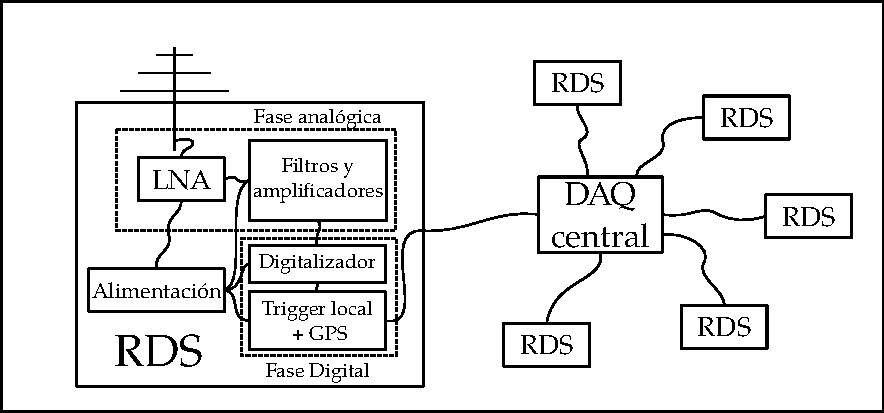
\includegraphics[width=\textwidth]{./fig/simulacionRadio/antennaSch}
			\caption{\label{fig:detectorSch} Esquema de un arreglo de antenas de radio gen\'erico.
			Cada estaci\'on de detecci\'on (RDS por \emph{Radio Detection Station}) es un elemento aut\'onomo del detector. Las componentes de su fase anal\'ogica son, la antena y un amplificador de bajo ruido (LNA por \emph{Low Noise Amplifier}) seguidos una serie de filtros y amplificadores. Luego, adem\'as de digitalizar la se\~nal se evaluan algoritmos de trigger locales y se agrega una etiqueta temporal mediante GPS.
			Finalmente, cada RDS se conecta a un sistema de adquisici\'on central (DAQ Central) que se encarga de discriminar eventos globales. M\'as informaci\'on en el texto.
			}
			
		\end{figure}
	%
	Si bien cada las componentes de cada RDS var\'ian de detector a detector, usualmente constan de una fase de detecci\'on anal\'ogica, una etapa de digitalizaci\'on y an\'alisis.
	\begin{enumerate}
		\item \textbf{Fase anal\'ogica:} esta etapa comienza en la antena. Una vez que el campo el\'ectrico genera un exceso de carga entre sus brazos, la corriente generada es amplificada por un amplificador de bajo ruido (LNA) que suele ubicarse a su pie, con el fin de evitar p\'erdidas. Luego, la se\~nal pasa por una segunda etapa de amplificaci\'on y filtrado y es transmitida hacia la fase digital.
		\item \textbf{Fase digital:} en este tramo la se\~nal es digitalizada, usualmente por un dispositivo ADC y analizada por un FPGA o un CPU. Este an\'alisis puede incluir la evaluaci\'on de niveles de disparo, el filtrado de frecuencias de ruido conocidas o incluso alguna transformaci\'on conveniente necesaria para el posterior an\'alisis. Una vez finalizada la etapa de tratamiento la se\~nal es almacenada junto a una etiqueta temporal normalmente obtenida mediante GPS. 
		Cada vez que una RDS cumple con todos los criterios de disparo locales, el tiempo de GPS de la se\~nal es enviado a un sistema de adquisici\'on central (DAQ Central) en el que se evaluan los niveles de disparo globales.
		Si estos se cumplen el DAQ Central indica a cada RDS del evento que envie la se\~nal almacenada para que sea guardada en disco.
	\end{enumerate}
	
	Como consecuencia de este proceso, la se\~nal alcanza la antena es diferente a la que finalmente es almacenada en el disco, donde el mayor impacto proviene del filtrado que se produce en la fase anal\'ogica a consecuencia de las respuestas en frecuencia de la antena y los amplificadores.
	Dado que estas respuestas pueden ser manejadas para satisfacer las necesidades del detector, en este trabajo se supondr\'a que cada RDS presenta una respuesta plana en frecuencia y adem\'as se se seleccionar\'a una banda particular, determinada por los siguientes factores:
	\begin{itemize}
	 \item La contaminaci\'on proveniente de la onda media predomina en la regi\'on \cant{0.2\text{-}30}{MHz}
	 \item La observaci\'on en frecuencias entre \cant{30\text{-}80}{MHz} es factible y actualmente utilizada por la mayor\'ia de los experimentos de radio actuales.
	 \item Las emisoras de FM ocupan la banda \cant{80\text{-}120}{MHz}
	 \item La se\~nal simulada de cascadas atmosf\'ericas en eventos ES muestra coherencia hasta el GHz.
	\end{itemize}
	
	Teniendo esto en cuenta, a la se\~nal simulada con \zhs{} se le aplicar\'a un filtro pasa banda \cant{30\text{-}80\text{/}120\text{-}900}{MHz} a las tres componentes del campo.
	
	Por otro lado, el hecho de conservar las tres componentes del campo el\'ectrico es un hecho no menor.
	Dado que su polarizaci\'on es paralela al frente de la lluvia (ver secci\'on \ref{sc:macroscopico}), la componente $z$ del campo el\'ectric\'o puede llegar a ser importante en lluvias inclinadas, al contrario de lo que sucede en eventos verticales.
	La figura \ref{fig:antSig} muestra el campo el\'ectrico obtenido mediante \zhs{}, medido en una antena ubicada sobre el anillo \cher{} para un evento ES que se dirige de Este a Oeste.
	Se grafican las componentes $z$, FW y TR del campo eléctrico, donde FW y TR son en la direcci\'on y transversal al movimiento del frente de la lluvia sobre el plano del suelo, respectivamente.
	
	%
	\begin{figure}[ht!]
		\centering
		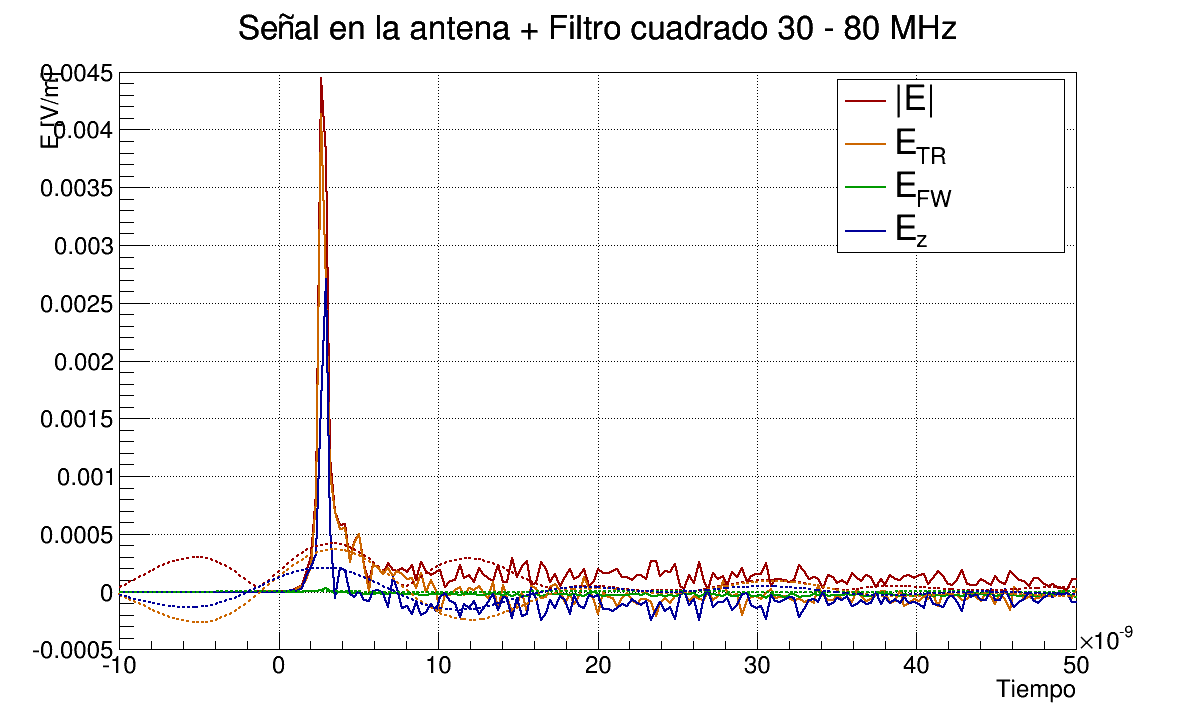
\includegraphics[width=0.8\textwidth]{./fig/simulacionRadio/antennaFilt}
		\caption{\label{fig:antSig}
		En l\'inea llena (punteada) se observa la señal en una antena ubicada a nivel del suelo sobre el anillo \cher{} antes (despu\'es) del filtrado en la banda \cant{30\text{-}80\text{/}120\text{-}900}{MHz}.  
		La componente FW del campo tiene la direcci\'on de propagaci\'on del frente de la lluvia sobre el plano del suelo, mientras que la componente TR es perpendicular a las componentes $z$ y FW.
		La ausencia de la componente FW es consistente con los modelos macrosc\'opicos expuestos en la secci\'on \ref{sc:macroscopico}.
		}
	\end{figure}
	
	\subsubsection{Evaluaci\'on del disparo local}
	\label{sbsc:localTriggerRadio}
	En un detector de radio real, la se\~nal que supera la etapa de digitalizaci\'on y alcanza la de evaluaci\'on de los niveles de disparo locales, se compone del pulso que se busca detectar y alg\'un nivel ruido.
	Por este motivo, existe siempre un campo incidente m\'inimo sobre la antena necesario para obtener una se\~nal detectable. 
	Esto es as\'i ya que la elecci\'on de los niveles de disparo locales se basa en un compromiso entre una relaci\'on se\~nal ruido alta \textbf{o} una eficiencia de disparo alta.
	Por este motivo, es necesario estudiar las fuentes de ruido que pueden afectar la medici\'on.
	
	La figura \ref{fig:allanNoise}, tomada de \cite{allan1971}, muestra los valores m\'inimos t\'ipicos que debe alcanzar el campo el\'ectrico en la antena para generar una se\~nal detectable, frente a diferentes fuentes de ruido y para un ancho de banda de \cant{1}{MHz}.
	%
	\begin{figure}[ht!]
		\centering
		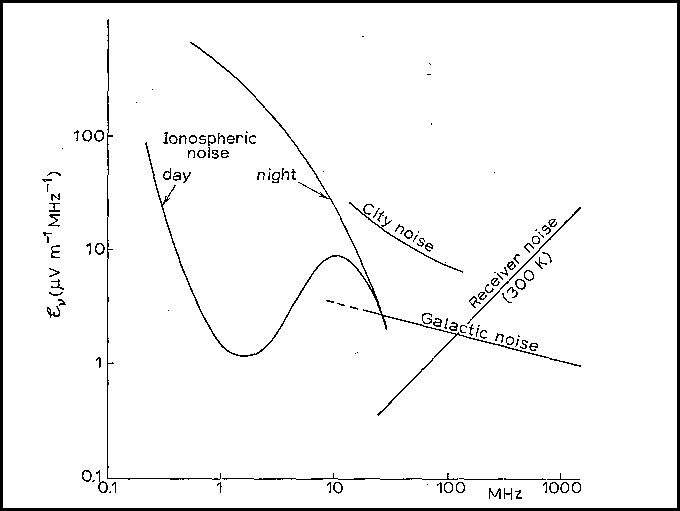
\includegraphics[width=0.8\textwidth]{./fig/simulacionRadio/allanNoise}
		\caption{\label{fig:allanNoise}
		Tomada de \cite{allan1971}. Niveles t\'ipicos de campo el\'ectrico m\'inimo detectable como funci\'on de la frecuencia, para diferentes niveles de ruido y un ancho de banda de \cant{1}{MHz}.
		En la banda \cant{30\text{-}80}{MHz} domina el ruido gal\'actico mientras que para la zona \cant{120\text{-}900}{MHz} lo hace el ruido intr\'inseco del receptor.
		}
	\end{figure}
	%
	Las posibles fuentes de ruido son las siguientes:
	%
	\begin{itemize}
	 \item \textbf{Ionosf\'erico:} la densidad de carga libre presente en la ion\'osfera provoca que act\'ue como un reflector para las ondas electromagn\'eticas en el rango \cant{100}{kHz}-\cant{30}{MHz}. De esta manera, es posible captar se\~nales originadas ya sea por emisoras de onda media o por tormentas a miles de kil\'ometros del lugar de observaci\'on.
	 \item \textbf{Proveniente de la ciudad:} el ruido electromagn\'etico presente en las ciudades, que proviene usualmente de aparatos industriales, suele ser el dominante en la mayor parte del ancho de banda si el receptor se encuentra dentro o cerca de la misma.
	 \item \textbf{Gal\'actico:} el ruido gal\'actico es todo aquel que proviene de fuentes extra terrestres (solar, c\'osmico o proveniente del plano gal\'actico). Este domina la regi\'on \cant{30\text{-}80}{MHz}, en ausencia de ruido humano.
	 \item \textbf{Intr\'inseco:} tambi\'en conocido como \emph{ruido de Johnson-Nyquist}, aparece en los terminales de la antena debido a fluctuaciones termodin\'amicas de los portadores de carga. Esta fuente depende de la temperatura de trabajo de la antena y se vuelve la fuente dominante por encima de de los \cant{100}{MHz}.
	\end{itemize}
	
	Entonces, idealmente el experimento deber\'a encontrarse lejos de las zonas pobladas para evitar el ruido proveniente de la ciudad.
	En estas condiciones el nivel de disparo local en la banda \cant{30\text{-}80\text{/}120\text{-}900}{MHz} depender\'a s\'olo del ruido gal\'actico y del intr\'inseco de la antena, donde ser\'a necesario llevar los valores de campo m\'inimo de la figura \ref{fig:allanNoise} al ancho de banda elegido.
	Para ello, es necesario tener en cuenta que la potencia del ruido es aditiva, es decir, $|E_\nu|^2\propto d\nu$, donde $E_\nu$ es campo el\'ectrico que genera la se\~nal en un ancho de banda $d\nu$.
	Por lo tanto el campo m\'inimo necesario en el ancho de banda seleccionado ser\'a:
	%
	\begin{equation}
	|E|_{min}=\left(\int_{30}^{80}(|E_\nu|^2_G+|E_\nu|^2_R)\,d\nu+
	\int_{120}^{900}(|E_\nu|^2_G+|E_\nu|^2_R)\,d\nu
	\right)^\frac{1}{2}
	\sim 250 {\rm\ \dfrac{\mu V}{m}}
	\end{equation}
	%
	donde $|E_\nu|_G$ y $|E_\nu|_R$ son los campos m\'inimos necesarios para superar el ruido gal\'actico y del receptor respectivamente, obtenidos a partir de la figura \ref{fig:allanNoise}.
	
	Por otra parte, si se tiene en cuenta que existen t\'ecnicas para erradicar el ruido del receptor, el campo m\'inimo en nuestro ancho de banda ser\'ia el necesario para superar el ruido gal\'actico:
	%
	\begin{equation}
	|E|_{min}=\left(\int_{30}^{80}|E_\nu|^2_G \,d\nu+
	\int_{120}^{900}|E_\nu|^2_G\, d\nu
	\right)^\frac{1}{2}
	\sim 40 {\rm\ \dfrac{\mu V}{m}}
	\end{equation}
	%
	
	Entonces, se evaluar\'a el disparo local de cada RDS sobre el m\'aximo del campo el\'ectrico simulado.
	Para ello, y con el fin de no perder generalidad en el resultado, se reportar\'a el resultado para diferentes niveles, entre \cant{25}{\frac{\mu V}{m}} y \cant{200}{\frac{\mu V}{m}} con un paso de \cant{25}{\frac{\mu V}{m}}.
	En el cap\'itulo \ref{ch:resultadosRadio} se mostrar\'a que el nivel de disparo local elegido, \'intimamente relacionado con la sensibilidad de la antena, es el factor limitante que m\'as afecta la exposici\'on obtenida.
	
	
\section{Caracterizaci\'on de eventos ES}

En esta secci\'on se realiza un recuento de las caracter\'isticas principales de la se\~nal de radio generada por lluvias ES.
Esto permitir\'a determinar el espacio de par\'ametros (energ\'ia, \'angulo cenital, etc) en el que este tipo de eventos prodr\'an ser detectados, y que por ende deber\'an ser simulados.

Para que un evento ES sea detectado, es necesario que se cumplan dos condiciones:
\begin{enumerate}
 \item La se\~nal de radio a nivel del suelo deber\'a ser lo suficientemente intensa y extensa para disparar varias antenas del detector, es decir, debe ser capaz de satisfacer ciertos criterios de disparo locales y globales.
 \item Las caracter\'isticas globales del evento deben permitir distinguirlo de los eventos de fondo, que al igual que en Auger son los generados por lluvias hadr\'onicas iniciadas cerca del tope de la atm\'osfera.
\end{enumerate}
por este motivo, en la subsiguiente caracterizaci\'on ser\'a clave determinar en qu\'e regi\'on del espacio de par\'ametros las condiciones 1 y 2 se cumplen.

	\subsection{Caracter\'isticas generales: evento típico}
	
	En esta direcci\'on, el primer paso en la caracterizaci\'on de la emisión de radio de un evento ES ser\'a estudiar lo que denominaremos un \emph{evento típico} o \emph{de referencia}, cuyas caracter\'isticas ser\'an utilizadas como punto de comparaci\'on al variar los parametros de la simulaci\'on. 
	A saber, las cualidades que definen la emisi\'on de radio de una lluvia ES en este an\'alisis son: 
	\begin{itemize}
	 \item el canal de decaimiento del \tauon{};
	 \item la energía transferida a la lluvia $E_v$, o energ\'ia visible\footnote{Se denomina energ\'ia visible de la lluvia a la acarreada por las part\'iculas interactuantes en del decaimiento del \tauon{}, es decir, la acarreada por electrones, positrones, fotones y hadrones, y que ser\'a transmitida r\'apidamente a las nuevas generaciones de part\'iculas. Por otro lado, la energ\'ia transferida a part\'iculas penetrantes, neutrinos y muones, se perder\'a debido a su baja frecuencia de interacci\'on.};
	 \item sus parámetros geométricos $(\theta,{\rm x_d},\phi)$;
	 \item la disposici\'on de las antenas;
	 \item la ubicaci\'on geogr\'afica del detector, que determina el campo geomagn\'etico.
	 
	\end{itemize}

	Es interesante destacar que a diferencia del calculo realizado para Auger, en este análisis las lluvias ES se caracterizarán por su energía visible $E_v$ y no por la energía del \tauon{} emergente.
	Esta elección minimiza la cantidad de simulaciones que deben realizarse si se cumplen ciertas hip\'otesis (ver secci\'on \ref{sbsc:decayChRadio}) y deberá ser tenida en cuenta a la hora de calcular la exposición del detector.
	
	Por otra parte, los par\'ametros que definen el evento t\'ipico se eligieron de manera que alcance un $100\%$ de eficiencia de disparo, como podr\'a corroborarse en el cap\'itulo \ref{ch:resultadosRadio}.
	Estos se muestran en la tabla \ref{tab:paramTestShower}.
	%
	\begin{table}[ht!]
	 \begin{center}
	  \begin{tabular}{|c|cccc|}
	   \hline
	   Canal de decaimiento & $E_v$ & $\theta$ & \xd{} & $\phi$ \\
	   \hline
	   $\tau\rightarrow e^- \nu_{e^-}\nu\tau$ & \cant{10^{18}}{eV} & \cant{90.5}{^\circ} & \cant{25}{m} & \cant{90}{^\circ} \\
	   \hline
	  \end{tabular}
	  \caption{\label{tab:paramTestShower}
	  Parámetros de simulación del \emph{evento típico} que se utilizará como referencia.
	  }
	 \end{center}
	\end{table}
	%
	
	Para estudiar el evento t\'ipico se simular\'a la se\~nal sobre un arreglo de antenas cuyo paso es \cant{1000}{m} en la dirección de propagación y \cant{100}{m} en la dirección transversal, en un arreglo de \cant{2\times80}{km}.
	Estos par\'ametros, que no tendr\'an nada que ver con la disposici\'on de las antenas del detector real, representan una buena relaci\'on de compromiso entre la granularidad con la que se mide la se\~nal y el tiempo de c\'omputo.
	
	Por \'ultimo es necesario elegir una ubicaci\'on para el detector. 
	Como se ha mencionado, el c\'alculo descripto en esta parte de la tesis no esta ligado a ning\'un experimento en particular, sin embargo, para elegir el sitio en el que se simular\'a el detector, se decidi\'o considerar s\'olo como ubicaciones en las que ya se encuentre funcionando algun detector de rayos c\'osmicos que utilize la t\'ecnica de radio.
	Entonces, las locaciones tenidas en cuenta se detallan en la tabla \ref{tab:possibleLoc} junto con las caracter\'isticas del campo geomagn\'etico promedio en sus inmediaciones (tomado de \cite{noaa}).
	%
	\begin{table}[ht!]
	\centering
	\footnotesize
	\newcolumntype{L}{>{\centering\arraybackslash}m{2.25cm}}
		\begin{tabular}{LLLLL}
		\toprule
		Experimento (Sitio) & Coordenadas & Declinaci\'on (+E,-W) & Inclinaci\'on (+D,-U)& Intensidad [Gauss] \\
		\midrule
		PAO Aera (Malarg\"ue Argentina) 
		& $35^\circ12$'${\rm S} $ $69^\circ18$'${\rm W}$
		& $(1.68\pm0.37)^\circ$ & $-36.3\pm0.22)^\circ$ & $0.2392\pm0.0015$ \\ \midrule
		Tunka Rex  (Tunka Valley Rusia) 
		& $51^\circ48$'${\rm N}$ $103^\circ04$'${\rm E}$
		& $(-2.82\pm0.37)^\circ$ & $(-71.2\pm0.22)^\circ$ & $0.6037\pm0.0015$ \\ \midrule
		Trend  (Tian shan China) 
		& $40^\circ32$'${\rm N}$ $78^\circ25$'${\rm E}$
		& $(3.76\pm0.37)^\circ$ & $(60.0\pm0.22)^\circ$ & $0.5391\pm0.0015$ \\
		\bottomrule
		\end{tabular}
		\caption{\label{tab:possibleLoc} Ubicaciones consideradas para el detector de radio junto a las caracter\'isticas del campo geomagn\'etico, tomadas de \cite{noaa}. Por su intensidad e inclinaci\'on, Tunka presenta el campo m\'as favorable para la detecci\'on de lluvias atmosf\'ericas inclinadas mediante t\'ecnicas de radio.}
	\end{table}
	
	De las tres posibles ubicaciones, Tunka posee el campo geomagn\'etico m\'as intenso y vertical\footnote{La inclinaci\'on presentada en la tabla \ref{tab:possibleLoc} es medida respecto del plano del suelo.}. 
	Dado que la contribuci\'on del efecto geomagn\'etico a la se\~nal generada depende del producto $\vec{\beta}\times\vec{B}$, ambas cualidades favorecen la detecci\'on de eventos inclinados.
	Por este motivo el sitio elegido para todas las sumulaciones fue Tunka.
	
	\subsubsection{Huella sobre el detector - Cono \cher}
	
	La primer caracter\'istica imporante de este tipo de eventos es la geometr\'ia de la huella dejada sobre el detector.
	La figura \ref{fig:testFootprint_Cone} muestra el módulo del máximo campo eléctrico registrado a nivel del suelo, luego de aplicarle a la se\~nal el tratamiento descripto en la secci\'on \ref{sbsc:sig_treat}.
	%
	\begin{figure}[ht!]
		\centering
		\includegraphics[width=\textwidth]{./fig/simulacionRadio/{foorPrint_Cone_ZWv1.22_ntuples_v1.21_ChTest_phi_90_18_89.5_90_25_1238_E0}.png}
		\caption{\label{fig:testFootprint_Cone}
		Huella de campo eléctrico generada por la lluvia ES típica. En rojo se muestra la zona de impacto del cono \cher{} si el máximo de la lluvia se encuentra a \cant{11}{km} del punto de decaimiento. Esta curva se obtuvo a partir de la ecuación \ref{eq:conewidth}, a la que se llegó mediante hipótesis geométricas.
		}
	\end{figure}
	%
	
	Hay tres aspectos muy importantes a destacar de esta figura.
	El primero es que, como se observa en línea roja, la zona de impacto del cono \cher{} predicha por la ecuación \ref{eq:conewidth} coincide con la huella de radio de manera notable.
	Para obtener la predicción se utilizaron los parámetros de la simulación para la altura de decaimiento y el ángulo cenital, mientras que la posición del máximo de la lluvia se obtuvo mediante prueba y error, pero utilizando valores razonables\footnote{El m\'aximo de una lluvia de \cant{10^{18}}{eV} se produce aproximadamente a \cant{10}{km} de la primera interacci\'on.}.
	Si bien \zhs{} realiza la simulación microscópicamente, es decir, sin realizar ninguna suposición sobre los mecanismos macrosc\'opicos, este resultado permite corroborar que la geometr\'ia emisi\'on de radio en eventos ES se explica a primer orden mediante razonamientos delineados en la sección \ref{sbsc:geom_emision}.
	
	La segunda observación es que en la dirección transversal a la de propagación el tamaño de la huella es de al rededor de \cant{2}{km}, es decir, las lluvias ES generan huellas muy alargadas sobre el detector, lo que se esperaba debido a que el \'angulo \cher{} es $\theta_{Cher}\sim1.4^\circ$.
	Si bien la poca apertura de la se\~nal en esta direcci\'on desfavorece su detecci\'on, es la característica fundamental a partir de la cual se pueden distinguír neutrinos ES de los eventos de fondo. 
	Esto es as\'i ya que los eventos inclinados que generan el background (eventos hadr\'onicos) se inician y desarrollan muy alto en la atmósfera y por ende generarán huellas de largo similar al de las lluvias ES, pero su ancho ser\'a mucho mayor debido a la apertura del cono \cher{}, cuyo v\'ertice se encuentra cerca del tope de la atm\'osfera.
	Este tema se volverá a abordar con mayor detalle en la sección \ref{sbsc:identificacionRadio}.
	 
	Por último, y en contraposición a lo anterior, en al dirección de propagación de la lluvia la huella alcanza niveles detectables (\cant{\gtrsim50}{\mu V/m}) en una zona de aproximadamente \cant{50}{km} de largo.
	Esta es una cualidad muy favorable a la hora detectar este tipo de eventos, ya que aumenta la probabilidad de disparar antenas, incluso donde las part\'iculas de la lluvia no alcanzan el suelo.
	Esto queda de manifiesto en la figura \ref{fig:sim_foot_y_part}, en la que se grafican las part\'iculas de la lluvia sobre la distribuci\'on del campo el\'ectrico de la lluvia.
	%
	\begin{figure}[ht!]
		\centering
		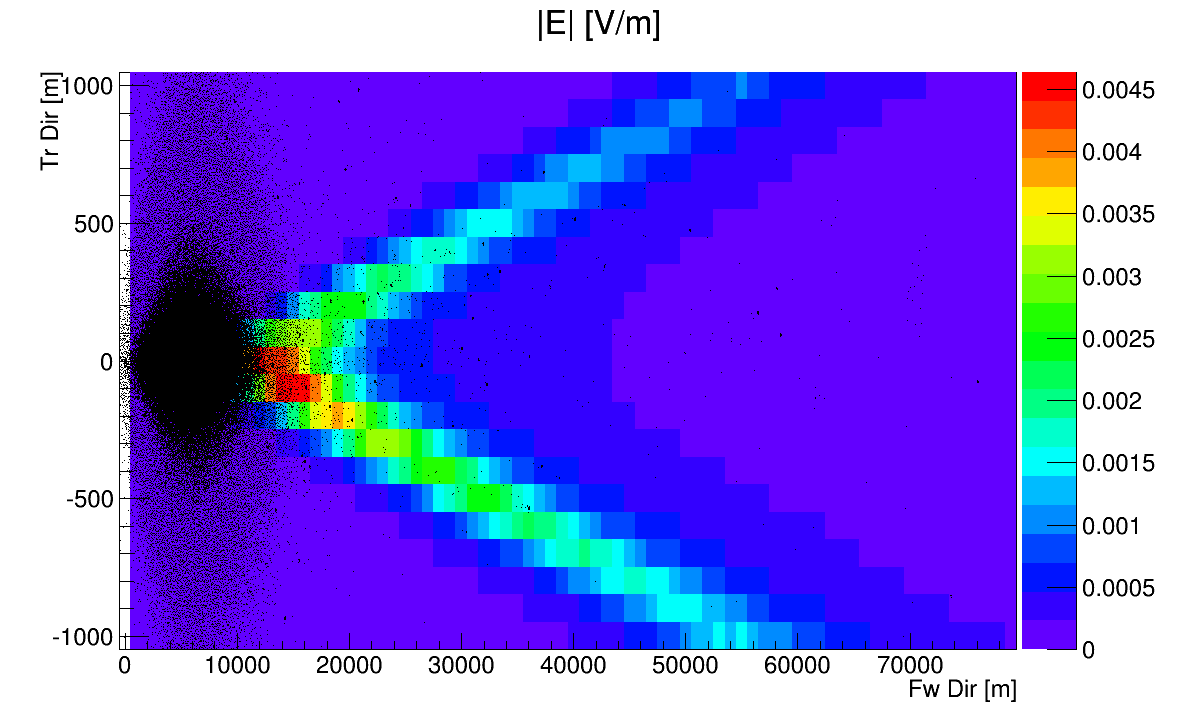
\includegraphics[width=\textwidth]{./fig/simulacionRadio/foorPrint_Test_18_89-5_90_25_1238_E_particles}
		\caption{\label{fig:sim_foot_y_part}
		Comparaci\'on entre la distribuci\'on de part\'iculas de la lluvia que alcanzan el suelo y la huella de campo el\'ectrico dejada en el detector.
		}
	\end{figure}
	
	\subsubsection{Polarización de la señal - Influencia del campo magn\'etico terrestre}
	
	Otra car\'acter\'istica de la se\~nal sobre el detector que vale la pena estudiar es la polarizaci\'on del campo el\'ectrico en cada una de las antenas, que podr\'a ser explicada a trav\'es de los modelos macrosc\'opicos delineados en el cap\'itulo \ref{easRadio}.
	Para ello se considerar\'a al evento de referencia como una lluvia completamente horizontal ($\theta=90^\circ$) y que se desplaza de Oeste a Este ($\phi=90^\circ$) a alguna altura respecto del suelo.
	Bajo estas condiciones, y suponiendo que el campo magn\'etico terrestre es el de Tunka, es posible determinar la polarizaci\'on de la se\~nal en diferentes regiones del suelo, lo que se muestra en la figura \ref{fig:malField}.
	%
	\begin{figure}[ht!]
		\centering
		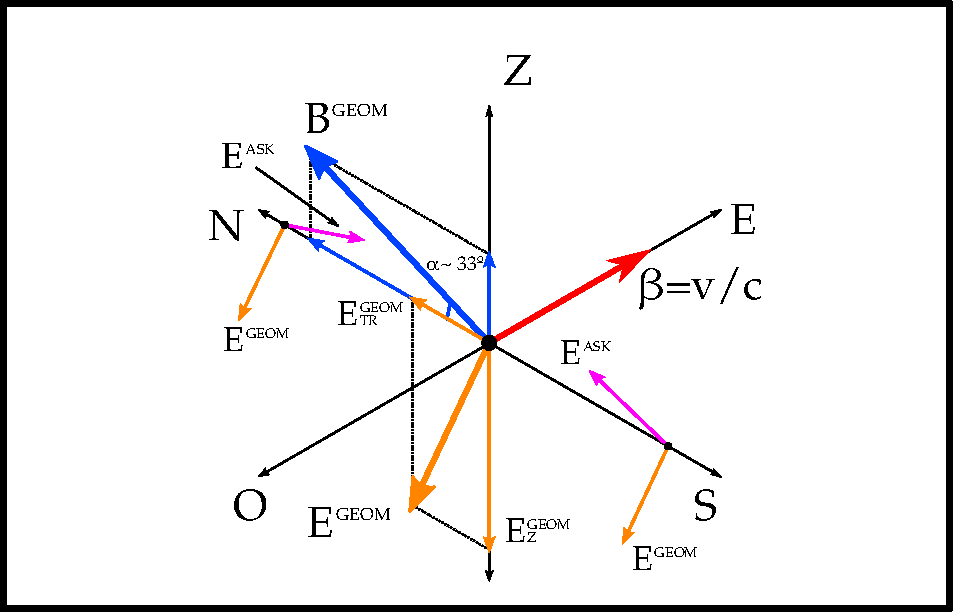
\includegraphics[width=0.8\textwidth]{./fig/simulacionRadio/malField}
		\caption{\label{fig:malField}
		Esquema de las componentes del campo elctrico para una lluvia que se desplaza de Oeste a Este en Tunka. Se considerarán los campos hacia arriba, o la componente $z$, y el campo transversal a la dirección de propagación de la lluvia sobre el suelo, componente ${\rm TR}$. Se desprecia por el momento la componente ${\rm FW}$, tambien sobre el suelo pero en la dirección de propagación. La contribución geomagnética conserva su dirección (transversal y hacia arriba) en todo el suelo. Por otro lado, el aporte del efecto Askaryan tiene una componentes transversales opuestas en el sector norte y el sur, mientras que la componente $z$ siempre es positiva.
		}
	\end{figure}
	%
	
	Por simplicidad es conveniente pensar en el campo en el sistema de referencia definido por la coordenada $z$ y las direcciónes paralela (${\rm FW}$) y transversal (${\rm TR}$) a la dirección de propagación sobre el suelo.
	Desde esta persectiva, a primer orden la contribución geomagnética al campo eléctrico tiene dirección $({\rm TR},z)$ ya que por construcción es perpendicular a la dirección de propagación.
	Por otro lado, a cada lado del eje de la lluvia la componente Askaryan tiene direcciones opuestas pero sobre el suelo siempre posee componente en $z>0$.
	
	En las figuras \ref{fig:testFootprint_E0tr} y \ref{fig:testFootprint_E0z} se grafican el campo en dirección ${\rm TR}$ y en dirección $z$ de la huella de la lluvia.
	%
	\begin{figure}[ht!]
		\centering
		\includegraphics[width=\textwidth]{./fig/simulacionRadio/{foorPrint_ZWv1.22_ntuples_v1.21_ChTest_phi_90_18_89.5_90_25_1238_E0x}.png}
		\caption{\label{fig:testFootprint_E0tr}
		Huella de campo eléctrico en la dirección ${\rm TR}$. La intensidad del cono \cher{} es distinta a ambos lados del eje de la lluvia.
		Cuando la coordenada transversal es positiva el efecto Askaryan y el geomagnético se suprimen mientras que cuando es negativa se favorecen.
		}
	\end{figure}
	%
	Como puede observarse en la figura \ref{fig:testFootprint_E0tr}, la intensidad del cono \cher{} no es simétrica respecto del eje de la lluvia.
	Esto se debe a que, como se esquematizó en la figura \ref{fig:malField}, en la parte norte de la lluvia las contribuciones Askaryan y geomagnética en la dirección ${\rm TR}$ se suprimen mientras que en la parte sur se favorecen.
	%
	\begin{figure}[ht!]
		\centering
		\includegraphics[width=\textwidth]{./fig/simulacionRadio/{foorPrint_ZWv1.22_ntuples_v1.21_ChTest_phi_90_18_89.5_90_25_1238_E0z}.png}
		\caption{\label{fig:testFootprint_E0z}
		Huella de campo eléctrico en la dirección $z$. En esta dirección las contribuciones geomagnética y Askaryan se suman en cualquier punto del suelo.
		}
	\end{figure}
	%
	Por otro lado, la componente $z$ del campo de ambas contribuciones no presenta ningun cambio de signo en el plano del suelo, lo que explica que la figura \ref{fig:testFootprint_E0z} muestre una huella mucho más simétrica respecto del eje generado por la direcci\'on de propagaci\'on.
	
	Por ultimo, hasta el momento se despreció la componente ${\rm FW}$. 
	Dado que las lluvias ES son casi horizontales la aparición de esta componente a nivel del suelo se vuelve despreciable, como se observa en la figura \ref{fig:testFootprint_E0fw} si se compara la intensidad de campo de la huella con la de las figuras \ref{fig:testFootprint_E0tr} y \ref{fig:testFootprint_E0z}.
	%
	\begin{figure}[ht!]
		\centering
		\includegraphics[width=\textwidth]{./fig/simulacionRadio/{foorPrint_ZWv1.22_ntuples_v1.21_ChTest_phi_90_18_89.5_90_25_1238_E0y}.png}
		\caption{\label{fig:testFootprint_E0fw}
		Campo eléctrico en la dirección ${\rm FW}$. Su intensidad es dos \'ordenes de magnitud menor que en las direcciones ${\rm TR}$ y $z$.
		}
	\end{figure}
	
	Dada la regularidad que presenta la polarizaci\'on a lo largo de toda la huella, puede ser explotada para eliminar de los eventos antenas con se\~nal esp\'urea.
	En la figura \ref{fig:footprintPolariz} se observa la distribuci\'on de \'angulo azimutal ($0^\circ$ hacia el norte) y cenital para las antenas cuya se\~nal supera el nivel de disparo.
	%
	\begin{figure}[ht!]
		\centering
		\includegraphics[width=\textwidth]{./fig/simulacionRadio/{phiDist2DColz_Test_18_89.5_90_25_1238}.png}
		\includegraphics[width=\textwidth]{./fig/simulacionRadio/{thDist2DColz_Test_18_89.5_90_25_1238}.png}
		\caption{\label{fig:footprintPolariz}
		Distribuci\'on de \'angulo azimutal y cenital a lo largo de la huella de la lluvia. Se observa que el \'angulo azimutal se mantiene en valores \emph{cercanos} a cero mientras que el cenital no presenta var\'ia entre $0^\circ$ y $90^\circ$.
		}
	\end{figure}
	%
	Se observa que el los valores de \'angulo azimutal se mantienen en valores cercanos a cero mientras que el \'angulo cenital var\'ia entre $0^\circ$ y $90^\circ$. 
	De aqu\'i, resulta natural imponer una restricci\'on a los valores de \'angulo azimutal que puede tomar la se\~nal de cada antena de un evento. 
	Para definirlo es resulta \'util la figura \ref{fig:phiDist}, que muestra la distribuci\'on de $\phi$ en forma de histograma. 
	%
	\begin{figure}[ht!]
		\centering
		\includegraphics[width=\textwidth]{./fig/simulacionRadio/{phiDist_Test_18_89.5_90_25_1238}.png}
		\caption{\label{fig:phiDist}
		Histograma del \'angulo azimutal del evento. Se distinguen las entradas procedentes de la zona norte (sur) de la huella en las que se observan valores levemente sesgados negativamente (positivamente). Se observa que la mayor\'ia de las antenas presentan valores entre $-2.5^\circ$ y $2.5^\circ$, lo que da una idea del \'orden de magnitud del rango angular a seleccionar.
		}
	\end{figure}
	%
	
	Si bien se observa que en la zona norte y sur de la huella presentan valores en promedio distintos, el valor absoluto se mantiene por debajo de $2.5^\circ$ en la mayor\'ia de los casos, lo que define una zona de aceptaci\'on de alrededor de $5^\circ$.
	Este valor permite entonces obtener una idea del orden de la reducci\'on en el numero de antenas con se\~nal esp\'urea. 
	Entonces, bajo la hip\'otesis de que la polarizaci\'on del ruido es aleatoria, la probabilidad de que una se\~nal esp\'urea aparezca en el rango definido por un evento sera $\sim 5/360\sim 1/60$.
	En resumen, un corte de selecci\'on en el \'angulo azimutal permitir\'ia rechazar alrededor del $98.5\%$ de las antenas disparadas por azar.
	
	
	\textbf{XXX ACA PODRIA AGREGAR lo de Bon y Boff y alguna evolucion del espectro o el espectro mismo}
	
	
	
% 	\begin{figure}[ht!]
% 		\centering
% 		\includegraphics[width=\textwidth]{./fig/simulacionRadio/{foorPrint_ZWv1.22_ntuples_v1.22_ChTest_phi_90_18_89.5_90_25_1238_E}.png}
% 		\includegraphics[width=\textwidth]{./fig/simulacionRadio/{foorPrint_ZWv1.22_ntuples_v1.22_ChTest_phi_90_18_89.5_90_25_1238_E0}.png}
% 		\caption{\label{fig:footprint_E_HEnv}
% 		asd
% 		}
% 	\end{figure}
% 	
% 	\begin{figure}[ht!]
% 		\centering
% 		\includegraphics[width=\textwidth]{./fig/simulacionRadio/{foorPrint_ZWv1.22_ntuples_v1.22_ChTest_phi_90_18_89.5_90_25_1238_EHB}.png}
% 		\includegraphics[width=\textwidth]{./fig/simulacionRadio/{foorPrint_ZWv1.22_ntuples_v1.22_ChTest_phi_90_18_89.5_90_25_1238_ELB}.png}
% 		\caption{\label{fig:footprint_HB-LB_HEnv}
% 		asd
% 		}
% 	\end{figure}
% 	
% 	\begin{figure}[ht!]
% 		\centering
% 		\includegraphics[width=\textwidth]{./fig/simulacionRadio/{foorPrint_ZWv1.22_ntuples_v1.22_ChTest_phi_90_18_89.5_90_25_1238_E}.png}
% 		\includegraphics[width=\textwidth]{./fig/simulacionRadio/{foorPrint_ZWv1.22_ntuples_v1.22_ChTest_phi_90_18_89.5_90_25_1238_E0}.png}
% 		\caption{\label{fig:footprint_E_HEnv}
% 		asd
% 		}
% 	\end{figure}
% 	
% 	\clearpage
	
	
	
% 	\begin{figure}[ht!]
% 		\centering
% 		\includegraphics[width=\textwidth]{./fig/simulacionRadio/{ZHSEvent_18_89.5_0_25_On_1238_E}.png}
% 		\includegraphics[width=\textwidth]{./fig/simulacionRadio/{ZHSEvent_18_89.5_0_25_Off_1238_E}.png}
% 		\caption{\label{fig:testFootprint_Ez}
% 		asd
% 		}
% 	\end{figure}
% 	
% 	\begin{figure}[ht!]
% 		\centering
% 		\includegraphics[width=\textwidth]{./fig/simulacionRadio/{ZHSEvent_18_89.5_0_25_On_1238_Ey}.png}
% 		\includegraphics[width=\textwidth]{./fig/simulacionRadio/{ZHSEvent_18_89.5_0_25_Off_1238_Ey}.png}
% 		\caption{\label{fig:testFootprint_Ez}
% 		asd
% 		}
% 	\end{figure}
% 	
% 	\begin{figure}[ht!]
% 		\centering
% 		\includegraphics[width=\textwidth]{./fig/simulacionRadio/{ZHSEvent_18_89.5_0_25_On_1238_Ez}.png}
% 		\includegraphics[width=\textwidth]{./fig/simulacionRadio/{ZHSEvent_18_89.5_0_25_Off_1238_Ez}.png}
% 		\caption{\label{fig:testFootprint_Ez}
% 		asd
% 		}
% 	\end{figure}
% 	
% 		\begin{figure}[ht!]
% 		\centering
% 		\includegraphics[width=\textwidth]{./fig/simulacionRadio/{ZHSEvent_18_89.5_0_25_On_1238_Ex}.png}
% 		\includegraphics[width=\textwidth]{./fig/simulacionRadio/{ZHSEvent_18_89.5_0_25_Off_1238_Ex}.png}
% 		\caption{\label{fig:testFootprint_Ez}
% 		asd
% 		}
% 	\end{figure}
% 	
% 	Bon y Boff
% 	
% 	mostrar que los efectos son comparables.
% 	
% 	velocidad de drift peque\~na por alra densidad en la atmósfera.
	
	
% 	\subsection{Evoluci\'on de la se\~nal a nivel del suelo}
% 		
% 	
% 	mostrar evolucion del EMax a lo largo de la lluvia
% 	
% 	mostrar espectro y evolucion
% 	
% 	mostrar fit del maximo de la lluvia como funcion de xd y theta y dependencia con la energia
% 	
% 		\subsubsection{Evoluci\'on de la polarizaci\'on}
% 		
% 		cambio askaryan geomagnetico?
	\clearpage
	
	\subsection{Caracterizaci\'on temporal}
	
	Velocidad de propagacion de la se\~nal.
	
	\subsection{Dependencia en los par\'ametros la lluvia}
	
	A fin de cuentas la exposici\'on a neutrinos depende de dos factores, las probabilidades de que se inicie una lluvia de par\'ametros dados y la eficiencia de detecci\'on e identificaci\'on de tales lluvias.
	Mientras que modificar las probabilidades de interacci\'on se encuentra fuera de alcance\footnote{Estas probabilidades dependen en gran medida del blanco con el que interact\'uan los neutrinos, que en este caso es la corteza de La Tierra.}, las eficiencias de detecci\'on pueden ser controladas en gran medida mediante el dise\~no del detector. 
	Es por esto que resulta clave entender c\'omo var\'ia la huella de radio de los eventos al variar los distintos par\'ametros de la lluvia.
	As\'i, a partir de este conocimiento y del estudio de las probabilidades de interacci\'on ser\'a posible optimizar el dise\~no del detector.
	
	Como se expuso en la secci\'on \ref{sbsc:localTriggerRadio}, la eficiencia de disparo de cada antena depende de del campo el\'ectrico m\'aximo registrado sobre la misma.
	Asimismo, el \'area sobre la cu\'al la huella de la radio supera el umbral de detecci\'on resulta ser una variable altamente relacionada con el disparo global de los eventos.
	En la misma l\'inea, el campo el\'ectrico m\'aximo registrado a lo largo de la huella permite inferir si un la lluvia tiene o no la capacidad de producir disparos locales.
	Por \'ultimo, como se ver\'a en la secci\'on \ref{sc:identificacionRadio} medidas del ancho de la huella se encuentran relacionadas con la posibilidad de distinguir eventos ES de las lluvias de fondo.
	Con todo esto en mente, en las siguientes secciones se estudiar\'a el comportamiento de algunas de estas variables al variar los par\'ametros del evento de referencia.
	
	\subsubsection{Efecto del \'angulo cenital $\theta$}
	
	En primer lugar se estudiar\'a c\'omo cambia la huella al variar el \'angulo cenital del evento.
	Debido a la geometr\'ia del cono \cher{} existir\'a un \'angulo m\'aximo a partir del cu\'al la emisi\'on de radio de la lluvia no interactuar\'a con el detector.
	Seg\'un el modelo simplificado presentado en la secci\'on \ref{sc:toymodelES} \'este \'angulo de corte deber\'ia ser $1.4^\circ$, como lo indica la figura \ref{fig:chConeWidth}.
	
	\begin{figure}[ht!]
		\centering
		\begin{tabular}{cc}
		$90.1^\circ$ & $90.5^\circ$ \\
		\includegraphics[width=0.5\textwidth]{./fig/simulacionRadio/theta/{foorPrint_ZWv1.21_ntuples_v1.21_Misc_phi_90_18_89.9_90_25_1238_E0}.png} &
		\includegraphics[width=0.5\textwidth]{./fig/simulacionRadio/theta/{foorPrint_ZWv1.21_ntuples_v1.21_Misc_phi_90_18_89.5_90_25_1238_E0}.png}\\
		
		$90.9^\circ$ & $91.3^\circ$ \\
		\includegraphics[width=0.5\textwidth]{./fig/simulacionRadio/theta/{foorPrint_ZWv1.21_ntuples_v1.21_Misc_phi_90_18_89.1_90_25_1238_E0}.png} &
		\includegraphics[width=0.5\textwidth]{./fig/simulacionRadio/theta/{foorPrint_ZWv1.21_ntuples_v1.21_Misc_phi_90_18_88.7_90_25_1238_E0}.png}\\
		
		$91.7^\circ$ & $92.3^\circ$ \\
		\includegraphics[width=0.5\textwidth]{./fig/simulacionRadio/theta/{foorPrint_ZWv1.21_ntuples_v1.21_Misc_phi_90_18_88.3_90_25_1238_E0}.png} &
		\includegraphics[width=0.5\textwidth]{./fig/simulacionRadio/theta/{foorPrint_ZWv1.21_ntuples_v1.21_Misc_phi_90_18_87.7_90_25_1238_E0}.png}\\
		\end{tabular}
		\caption{\label{fig:theta_dependence}
		Huella sobre el detector del evento de referencia, para diferentes \'angulos cenitales. En todos los casos la lluvia se inici\'o en $(x,y)=(0,0)$. Se observa como al aumentar el \'angulo cenital el punto de impacto del cono \cher{}
		(que se encuentra determinado aproximadamente por la antena con m\'axima se\~nal)
		se aleja del punto de inicio de la lluvia, en acuerdo con la figura \ref{fig:chConeWidth} del cap\'itulo \ref{ch:easRadio}. Por otro lado, es posible notar como el m\'aximo de la huella disminuye dos \'ordenes de magnitud al variar cerca de $2.5^\circ$ de \'angulo cenital.
		}
	\end{figure}
	
	La figura \ref{fig:theta_dependence} muestra la huella dejada sobre el detector por el evento de referencia con distintos \'angulos ceintales.
	Dado que en todos los casos la lluvia se inici\'o en $(x,y)=(0,0)$, el punto de impacto del cono \cher{} se desplaza hacia valores positivos de $x$ a medida que $\theta$ crece.
	En particular, para valores superiores a $\sim91.3^\circ$ la se\~nal que alcanza el detector no es coherente, lo que genera un corte en la eficiencia de detecci\'on.
	Para apoyar este punto en la figura \ref{fig:theta_dependence2} se muestra el campo el\'ectrico m\'aximo de la lluvia para diferentes \'angulos cenitales y energ\'ias.
	%
	\begin{figure}[ht!]
		\centering
		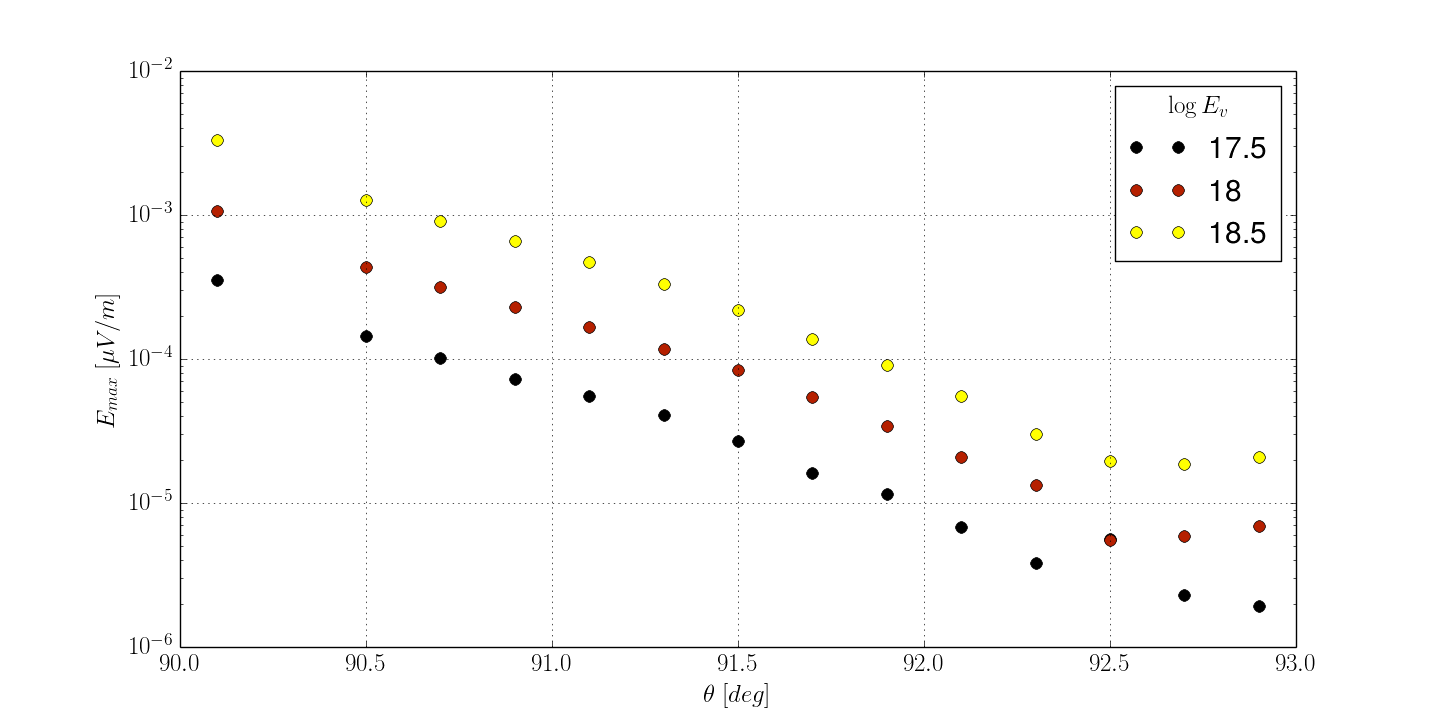
\includegraphics[width=\textwidth]{./fig/simulacionRadio/maxDep/eMaxTh}
		\caption{\label{fig:theta_dependence2}
		M\'aximo campo el\'ectrico de la lluvia como funci\'on del \'angulo cenital, para distintos valores de \ev{}. El decaimiento es aproximadamente exponencial.
		}
	\end{figure}
	%
	\textbf{Para una se observa como el campo decae exponencialmente hasta }
	
	Este fen\'omeno determina un \'anguo de corte a partir del cual la eficiencia de detecci\'on ser\'a practicamente nula\footnote{Si la coherencia de la se\~nal es baja el campo el\'ectrico m\'aximo ser\'a peque\~no y por ende la se\~nal no superar\'a los umbrales de detecci\'on.}.
	Por este motivo no se simular\'an eventos cuyo \'angulo cenital supere los $\sim91.5^\circ$.
	
	\subsubsection{Efecto de altura de decaimiento del tauon \xd{}}
	
	Tambien resulta interesante estudiar como cambia la huella del campo el\'ectrico al variar la altura de decaimiento del \tauon{} en el evento de referencia.
	Esto se muestra en la figura \ref{fig:xd_dependence} para \cant{xd = \left\{25,75,150,300\right\}}{m}, donde nuevamente la cascada se inici\'o en $(x,y)=(0,0)$.
	%
	\begin{figure}[ht!]
		\centering
		\begin{tabular}{cc}
		\cant{25}{m} & \cant{75}{m} \\
		\includegraphics[width=0.5\textwidth]{./fig/simulacionRadio/xd/{foorPrint_ZWv1.21_ntuples_v1.21_Misc_TestXd_18_89.5_90_25_1238_E0}.png} &
		\includegraphics[width=0.5\textwidth]{./fig/simulacionRadio/xd/{foorPrint_ZWv1.21_ntuples_v1.21_Misc_TestXd_18_89.5_90_75_1238_E0}.png}\\
		
		\cant{150}{m} & \cant{300}{m} \\
		\includegraphics[width=0.5\textwidth]{./fig/simulacionRadio/xd/{foorPrint_ZWv1.21_ntuples_v1.21_Misc_TestXd_18_89.5_90_150_1238_E0}.png} &
		\includegraphics[width=0.5\textwidth]{./fig/simulacionRadio/xd/{foorPrint_ZWv1.21_ntuples_v1.21_Misc_TestXd_18_89.5_90_300_1238_E0}.png}\\
		\end{tabular}
		\caption{\label{fig:xd_dependence}
		Huella sobre el detector del evento de referencia para distintas alturas de decaimiento. Se observa como a medida que aumenta la altura de decaimiento del \tauon{} la intensidad del campo el\'ectrico decrece.
		}
	\end{figure}
	Se observa como a medida que \xd{} aumenta la huella se traslada hacia valores positivos de $x$, lo que resulta nuevamente compatible con el modelo del cono \cher{}, en el que el plano de corte (la superficie de la tierra) se aleja paralelamente de su inicio.
	Cabe destacar que adem\'as de desplazarse, la intensidad de la huella disminuye a medida que aumenta \xd{}
	Esto puede observarse con mayor claridad en la figura \ref{fig:xd_dependence2}, que muestra como var\'ia el m\'aximo campo el\'ectrico registrado en la lluvia para diferentes valores de altura de decaimiento y energ\'ia visible.
	Se observa como a medida que \xd{} aumenta el campo decae de manera aproximadamente exponencial.
	%
	\begin{figure}[ht!]
		\centering
		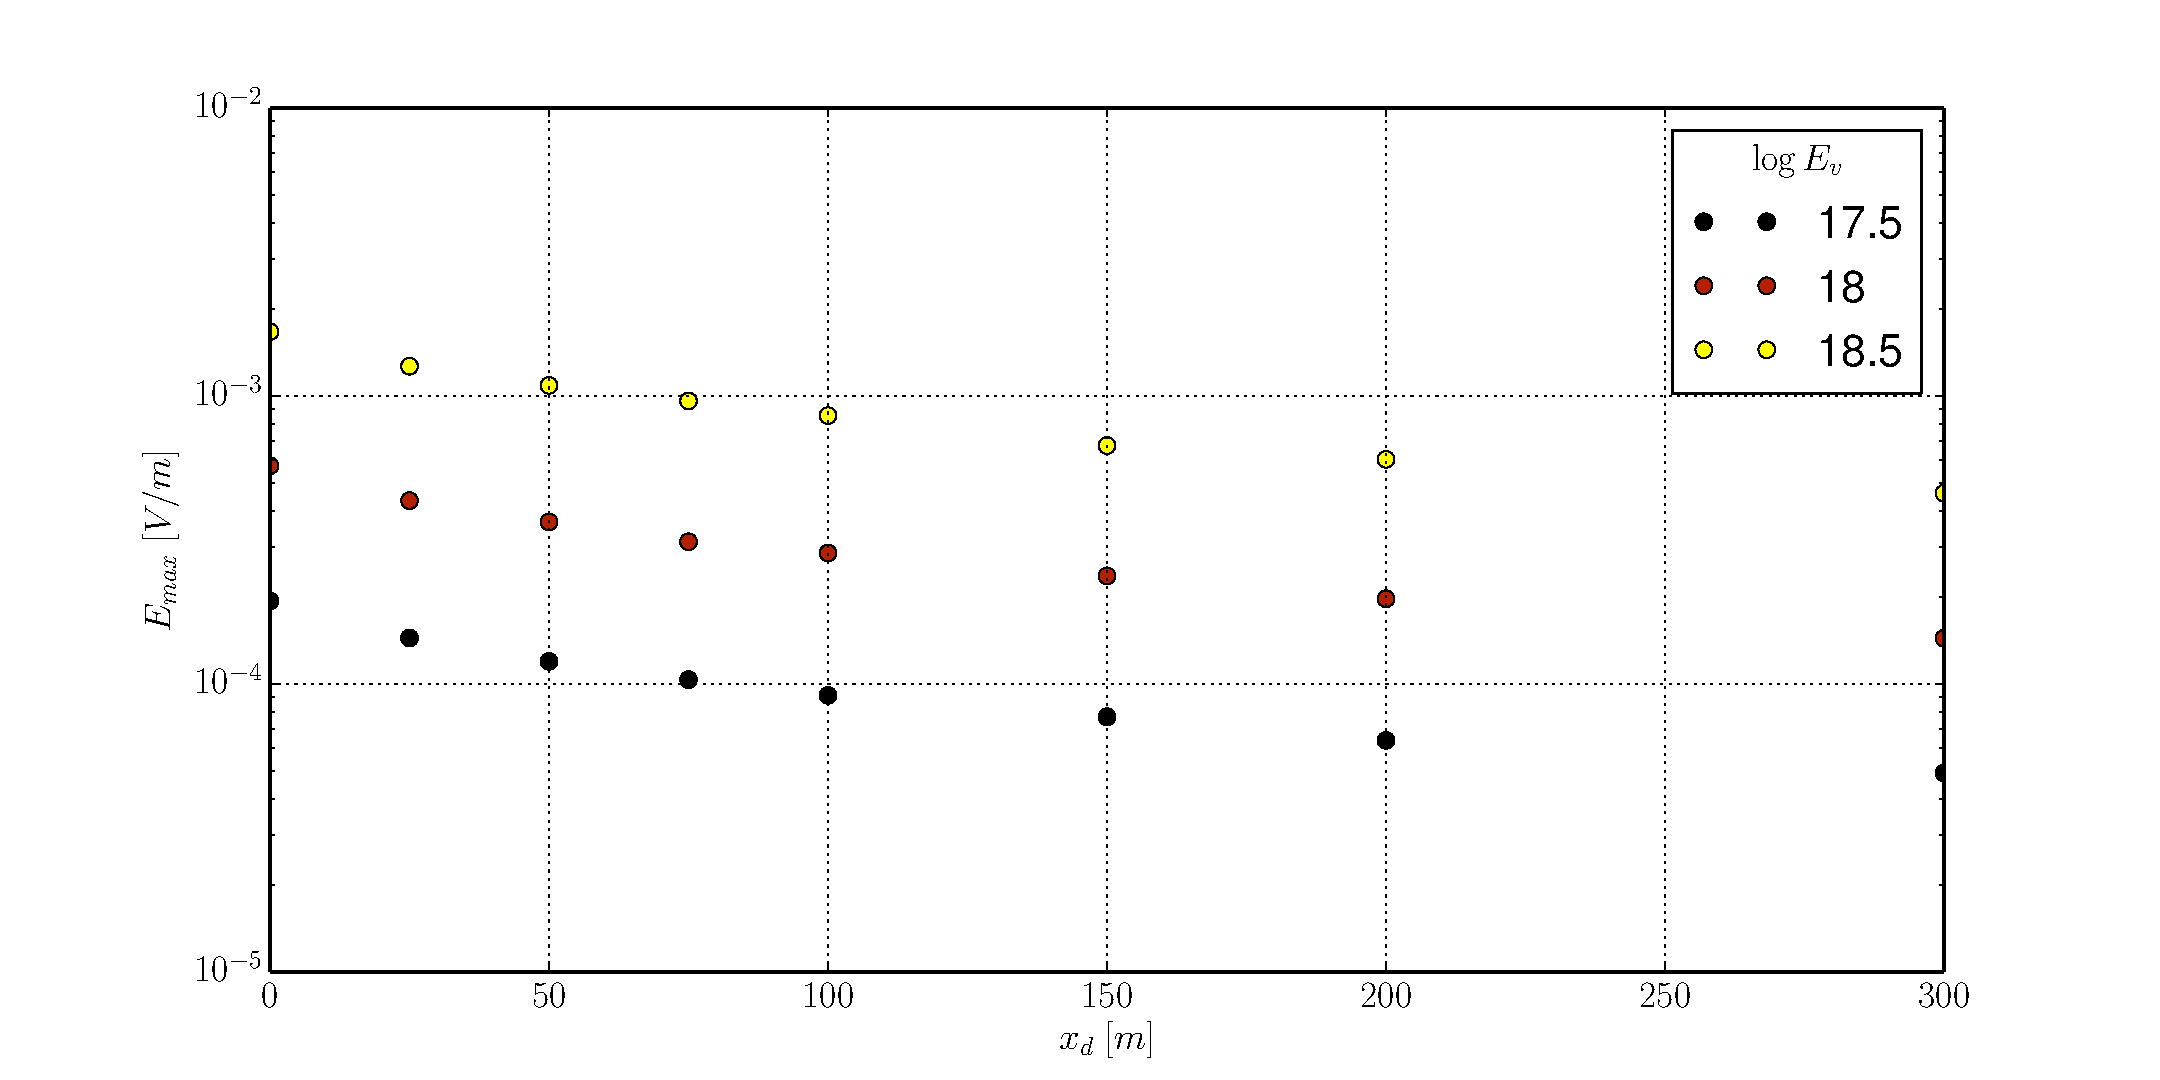
\includegraphics[width=\textwidth]{./fig/simulacionRadio/maxDep/eMaxXd}
		\caption{\label{fig:xd_dependence2}
		M\'aximo campo el\'ectrico de la lluvia como funci\'on de la altura de decaimiento del \tauon{}, para diferentes energ\'ias.
		Se observa un decaimiento aproximadamente exponencial.
		}
	\end{figure}
	
	Todo esto indica que existe una altura de decaimiento a partir de la cual los eventos dejer\'an de ser detectables. 
	Como se ver\'a mas adelante, este efecto tendr\'a importancia s\'olo a baja energ\'ia, mientras que para energ\'ias superioras a \cant{\sim10^{18}}{eV} la eficiencia a altos \xd{} se ver\'a suprimida por el efecto de la curvatura de la tierra (ver ap\'endice \ref{ap:tierraCurva} y cap\'itulo \ref{ch:resultadosRadio}).
	
	\subsubsection{Efecto del \'angulo azimutal $\phi$}
	
	En base a lo estudiado en el cap\'itulo \ref{ch:easRadio}, el efecto geomagn\'etico provoca que la distribuci\'on de campo el\'ectrico a nivel del suelo dependa del \'angulo azimutal.
	Para comprender mejor esta dependencia es interesante estudiar el t\'ermino $E(\phi)\propto\vec\beta(\phi)\times \vec B$ en Tunka\footnote{La declinaci\'on del campo geomagn\'etico en Tunka es de $71.2^\circ$.}.
	La figura \ref{fig:geomComps_Tunka} muestra la variaci\'on de las componentes $E_x$, $E_y$, $E_z$, $E_{TR}$ y $|E|$ con el \'angulo azimutal para un \'angulo cenital de $\theta=90.5^\circ$.
	%
	\begin{figure}[ht!]
		\centering
		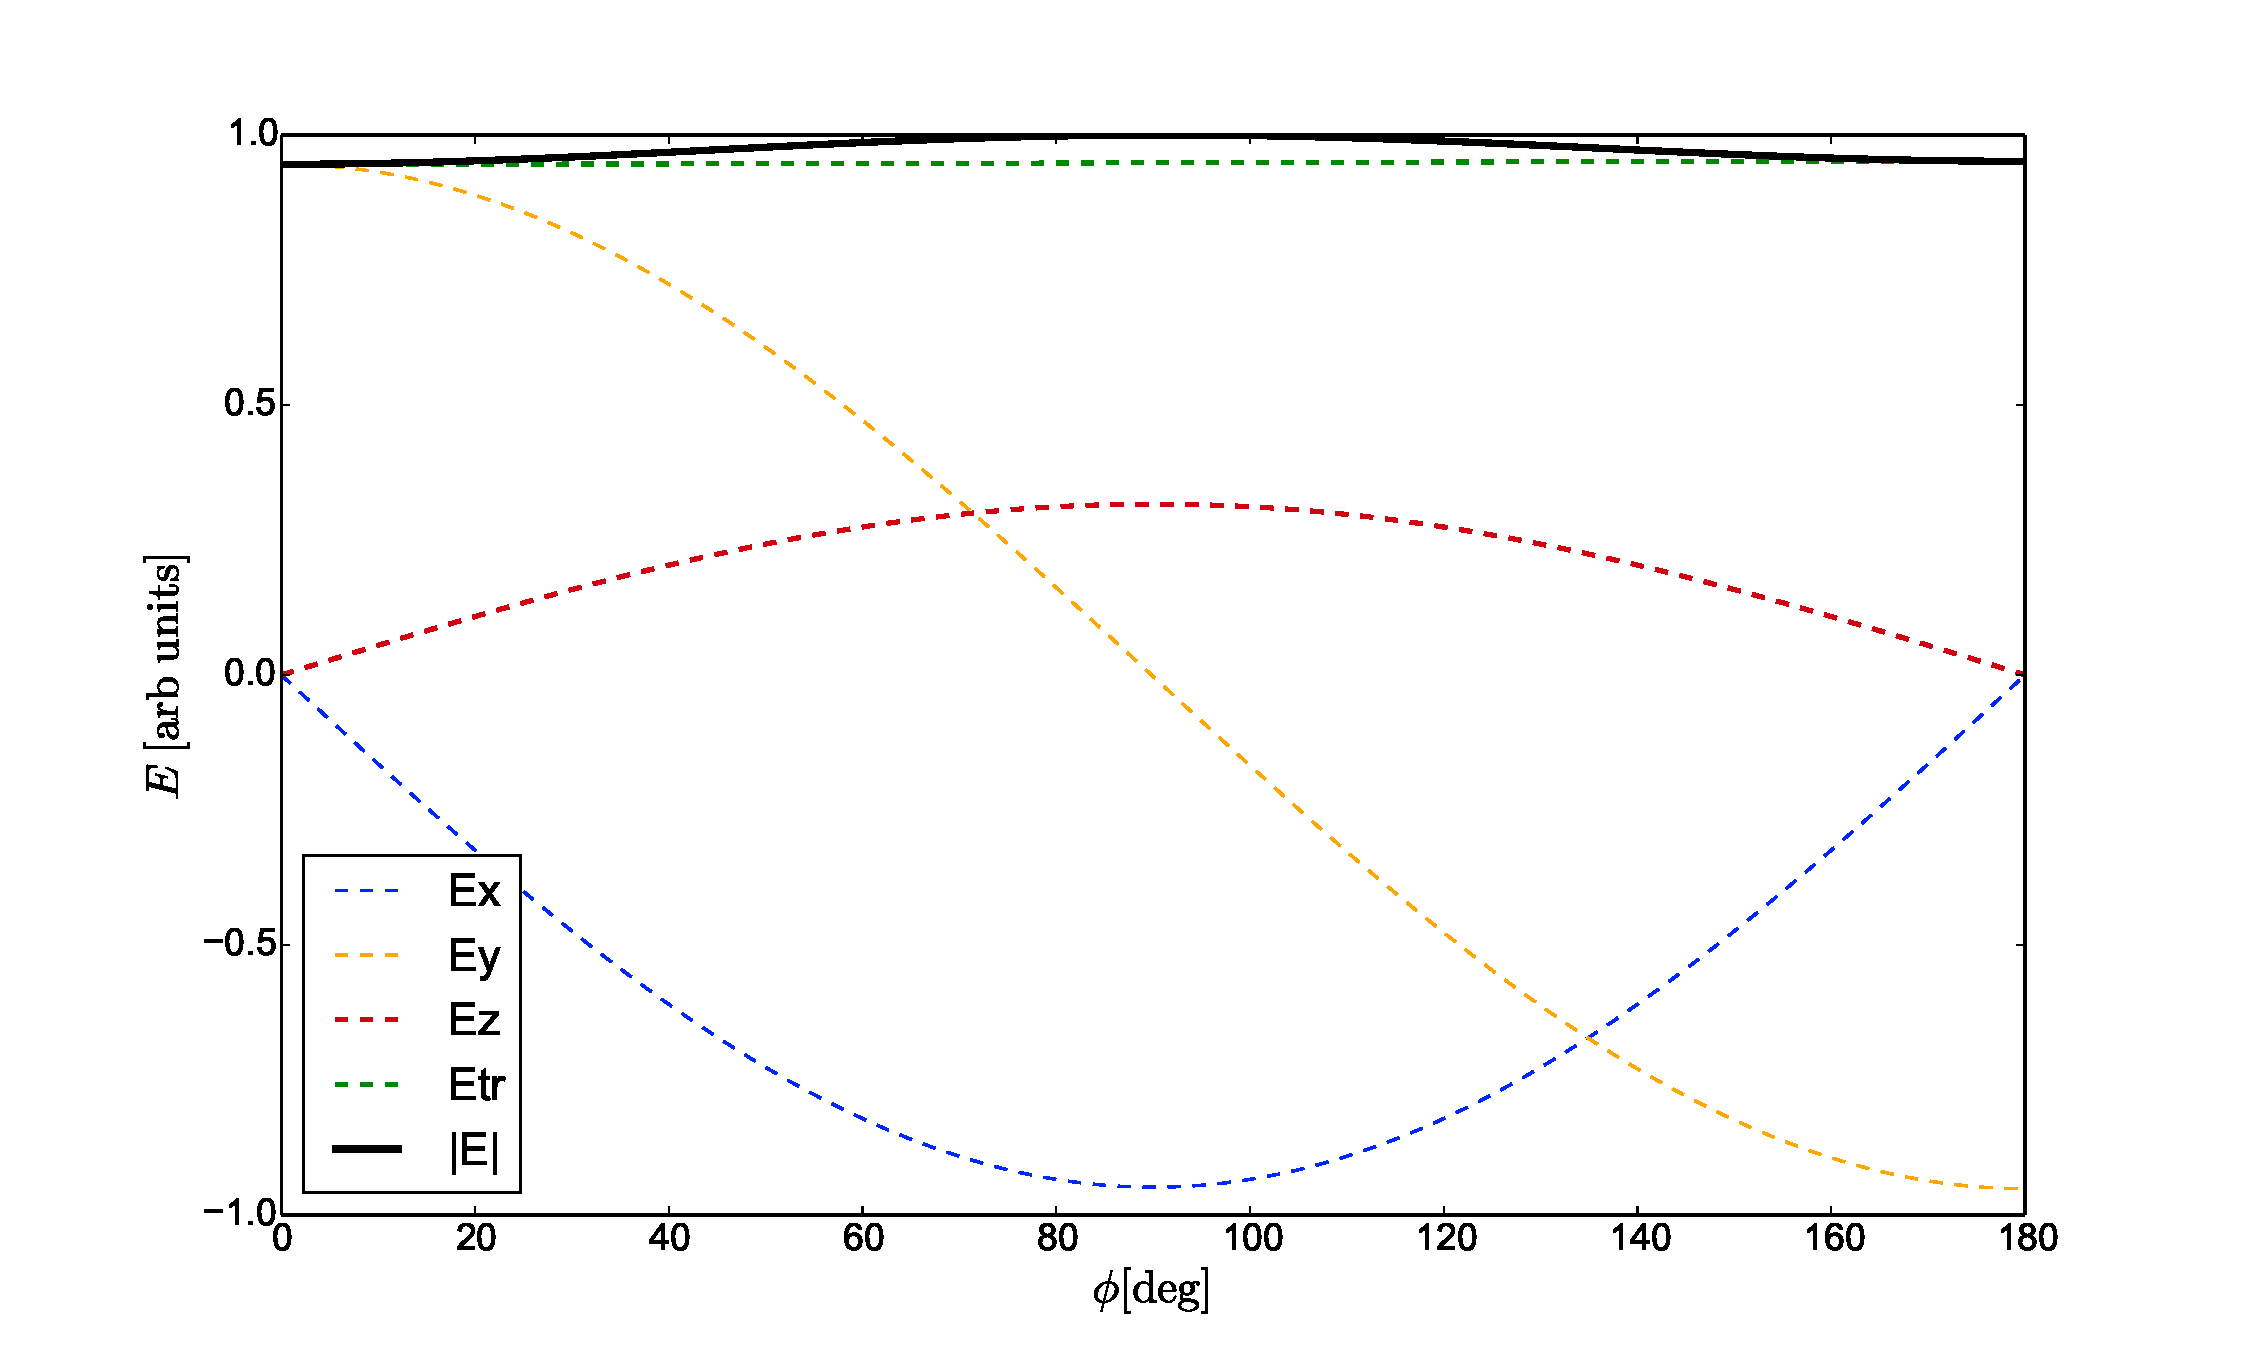
\includegraphics[width=\textwidth]{./fig/simulacionRadio/geomComps_Tunka}
		\caption{\label{fig:geomComps_Tunka}
		Componentes $E_x$, $E_y$, $E_z$, $E_{TR}$ y $|E|$ en funci\'on del \'angulo azimutal 
		$\phi$, calculados a partir de la ecuaci\'on $E(\phi)\propto\vec\beta(\phi)\times \vec B$. El campo geomagn\'etico utilizado tiene la declinaci\'on que se observa en Tunka,$71.2^\circ$. 
		}
	\end{figure}
	%
	Debido a que el campo geomagn\'etico en Tunka es casi vertical, si bien las componentes $E_x$ y $E_y$ var\'ian significativamente con $\phi$, la componente transversal $E_{TR}$ del campo se mantiene practicamente constante, lo que se observa en l\'inea de trazos verde. 
	Esto se debe a que esta componente depende b\'asicamente de la proyecci\'on vertical del campo geomagn\'etico.
	La peque\~na variaci\'on que se aprecia aparece debido a que el c\'alculo se realiz\'o suponiendo una lluvia no horizontal.
	Por otro lado, esta verticalidad en $\vec B$ provoca que para lluvias cuasi-horizontales, la coponente $E_z$ sea 0 para $\phi=0^\circ$ y $\phi=180^\circ$, y tome un valor m\'aximo para $\phi=90^\circ$, lo que se dibuja en l\'inea de trazos roja. 
	Como resultado de estas dos constribuciones, el m\'odulo total del campo el\'ectrico $|E|$ muestra una variaci\'on de aproximadamente $10\%$ entre 0 y 180 grados. 
	
	Con esto en mente resulta interesante entonces observar como se modifica la huella de $|E|$ del evento de referencia al cambiar el \'angulo azimutal entre $\phi=0^\circ$ y $\phi=90^\circ$, lo que se muestra para el evento de referencia en la figura \ref{fig:phi_dependence}. 
	\begin{figure}[ht!]
		\centering
		\begin{tabular}{cc}
		$0^\circ$ & $90^\circ$ \\
		\includegraphics[width=0.5\textwidth]{./fig/simulacionRadio/phi/{foorPrint_ZWv1.21_ntuples_v1.21_Misc_TestPhi_18_89.5_0_25_1238_E0}.png} &
		\includegraphics[width=0.5\textwidth]{./fig/simulacionRadio/phi/{foorPrint_ZWv1.21_ntuples_v1.21_Misc_TestPhi_18_89.5_90_25_1238_E0}.png}\\
		
		\end{tabular}
		\caption{\label{fig:phi_dependence}
		Huella sobre el detector del evento de referencia para $\phi=0^\circ$ y $\phi=90^\circ$.
		}
	\end{figure}
	En acuerdo con la figura \ref{fig:geomComps_Tunka} la huella para $\phi=0^\circ$ en promedio valores de campo el\'ectrico menores que para $\phi=90^\circ$, sin embargo, la variaci\'on a lo largo de la huella resulta mayor a $10\%$.
	Esta diferencia puede deberse a que el cambio de direcci\'on de la contribuci\'on del efecto geomagn\'etico provoque una cancelaci\'on con la contribuci\'on Askaryan.
	
	\subsubsection{Efecto de la eneg\'ia visible $E_v$}
	
	De acuerdo con lo expuesto en el cap\'itulo \ref{ch:easAuger} y en particular en la ecuaci\'on \ref{hi4}, el n\'umero de part\'iculas en el m\'aximo de la lluvia escala con la energ\'ia del primario o, el par\'ametro equivalente en eventos ES, la energ\'ia visible \ev{}.
	Por otra parte, dado que la emisi\'on de radio depende directamente del n\'umero de part\'iculas en el m\'aximo de la lluvia, resulta razonable suponer que la intensidad del campo el\'ectrico a nivel del suelo variar\'a tambien proporcionalmente a \ev{}.
	Para estudiar este efecto, en la figura \ref{fig:ev_dependence} se muestra la huela dejada por el evento de referencia con \cant{E_v=\left\{10^{17.5},10^{18},10^{18.5}\right\}}{eV}.
	Nuevamente el punto de inicio de la lluvia es $(x,y)=(0,0)$, y puede observarse como el campo el\'ectrico aumenta en intensidad a medida que aumenta la energ\'ia visible.
	%
	\begin{figure}[ht!]
		\centering
		\begin{tabular}{cc}
		\cant{10^{17.5}}{eV} & \cant{10^{18}}{eV}\\
		\includegraphics[width=0.5\textwidth]{./fig/simulacionRadio/ev/{foorPrint_ZWv1.21_ntuples_v1.21_Misc_TestEv_17.5_89.5_90_25_1238_E0}.png} &
		\includegraphics[width=0.5\textwidth]{./fig/simulacionRadio/ev/{foorPrint_ZWv1.21_ntuples_v1.21_Misc_TestEv_18_89.5_90_25_1238_E0}.png}\\
		
		\multicolumn{2}{c}{\cant{10^{18.5}}{eV}} \\
		\multicolumn{2}{c}{\includegraphics[width=0.5\textwidth]{./fig/simulacionRadio/ev/{foorPrint_ZWv1.21_ntuples_v1.21_Misc_TestEv_18.5_89.5_90_25_1238_E0}.png}}\\
		
		\end{tabular}
		\caption{\label{fig:ev_dependence}
		Huella sobre el detector del evento de referencia con \cant{E_v=\left\{10^{17.5},10^{18},10^{18.5}\right\}}{eV}.
		Se observa como a medida que aumenta \ev{} la intensidad del campo el\'ectrico aumenta.
		}
	\end{figure}
	
	Para reforzar la idea la figura \ref{fig:ev_dependence2} muestra como var\'ia el m\'aximo campo el\'ectrico de la lluvia con la energ\'ia para diversos valores de \'angulos cenitales y alturas de decaimiento.
	%
	\begin{figure}[ht!]
		\centering
		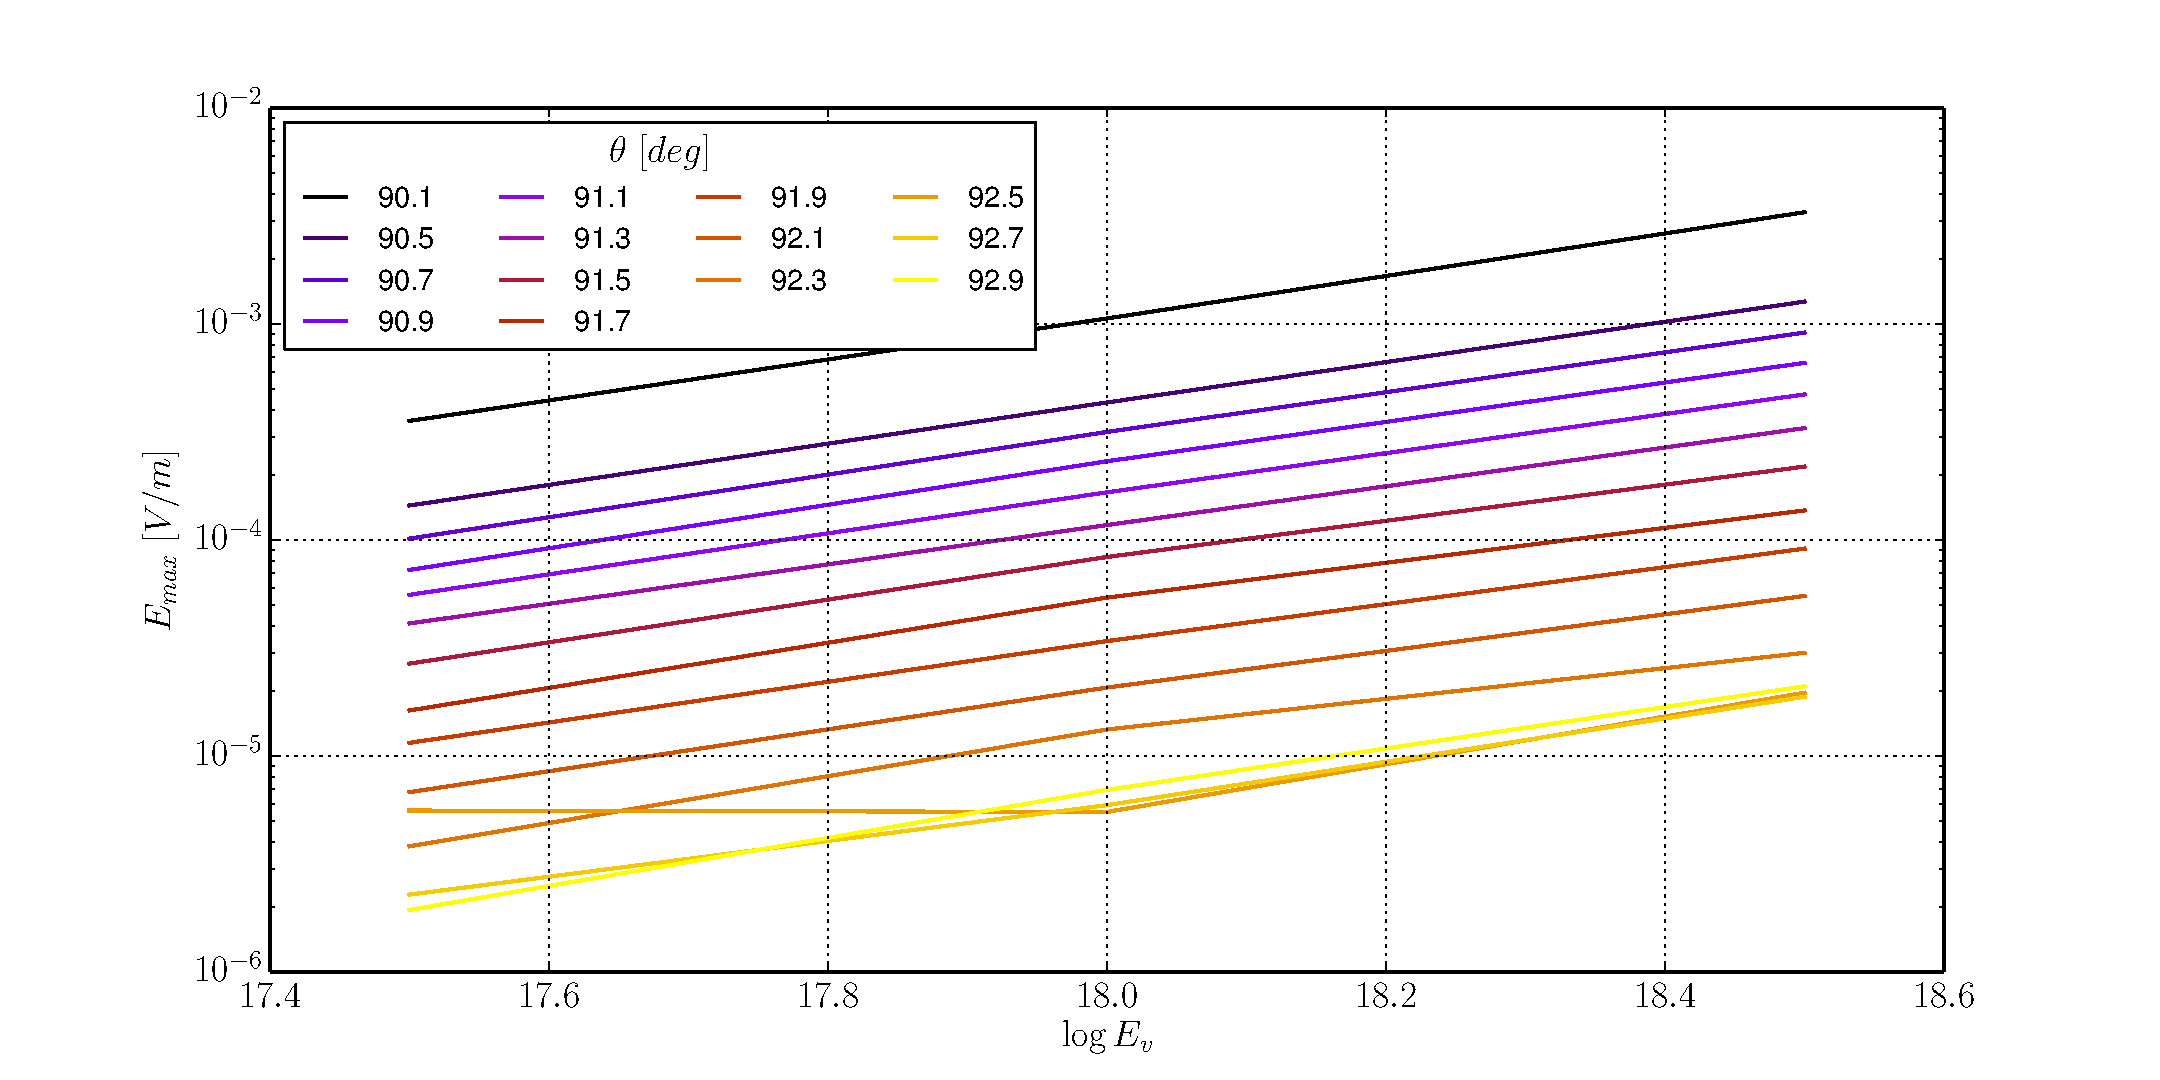
\includegraphics[width=\textwidth]{./fig/simulacionRadio/maxDep/eMaxThEv}
		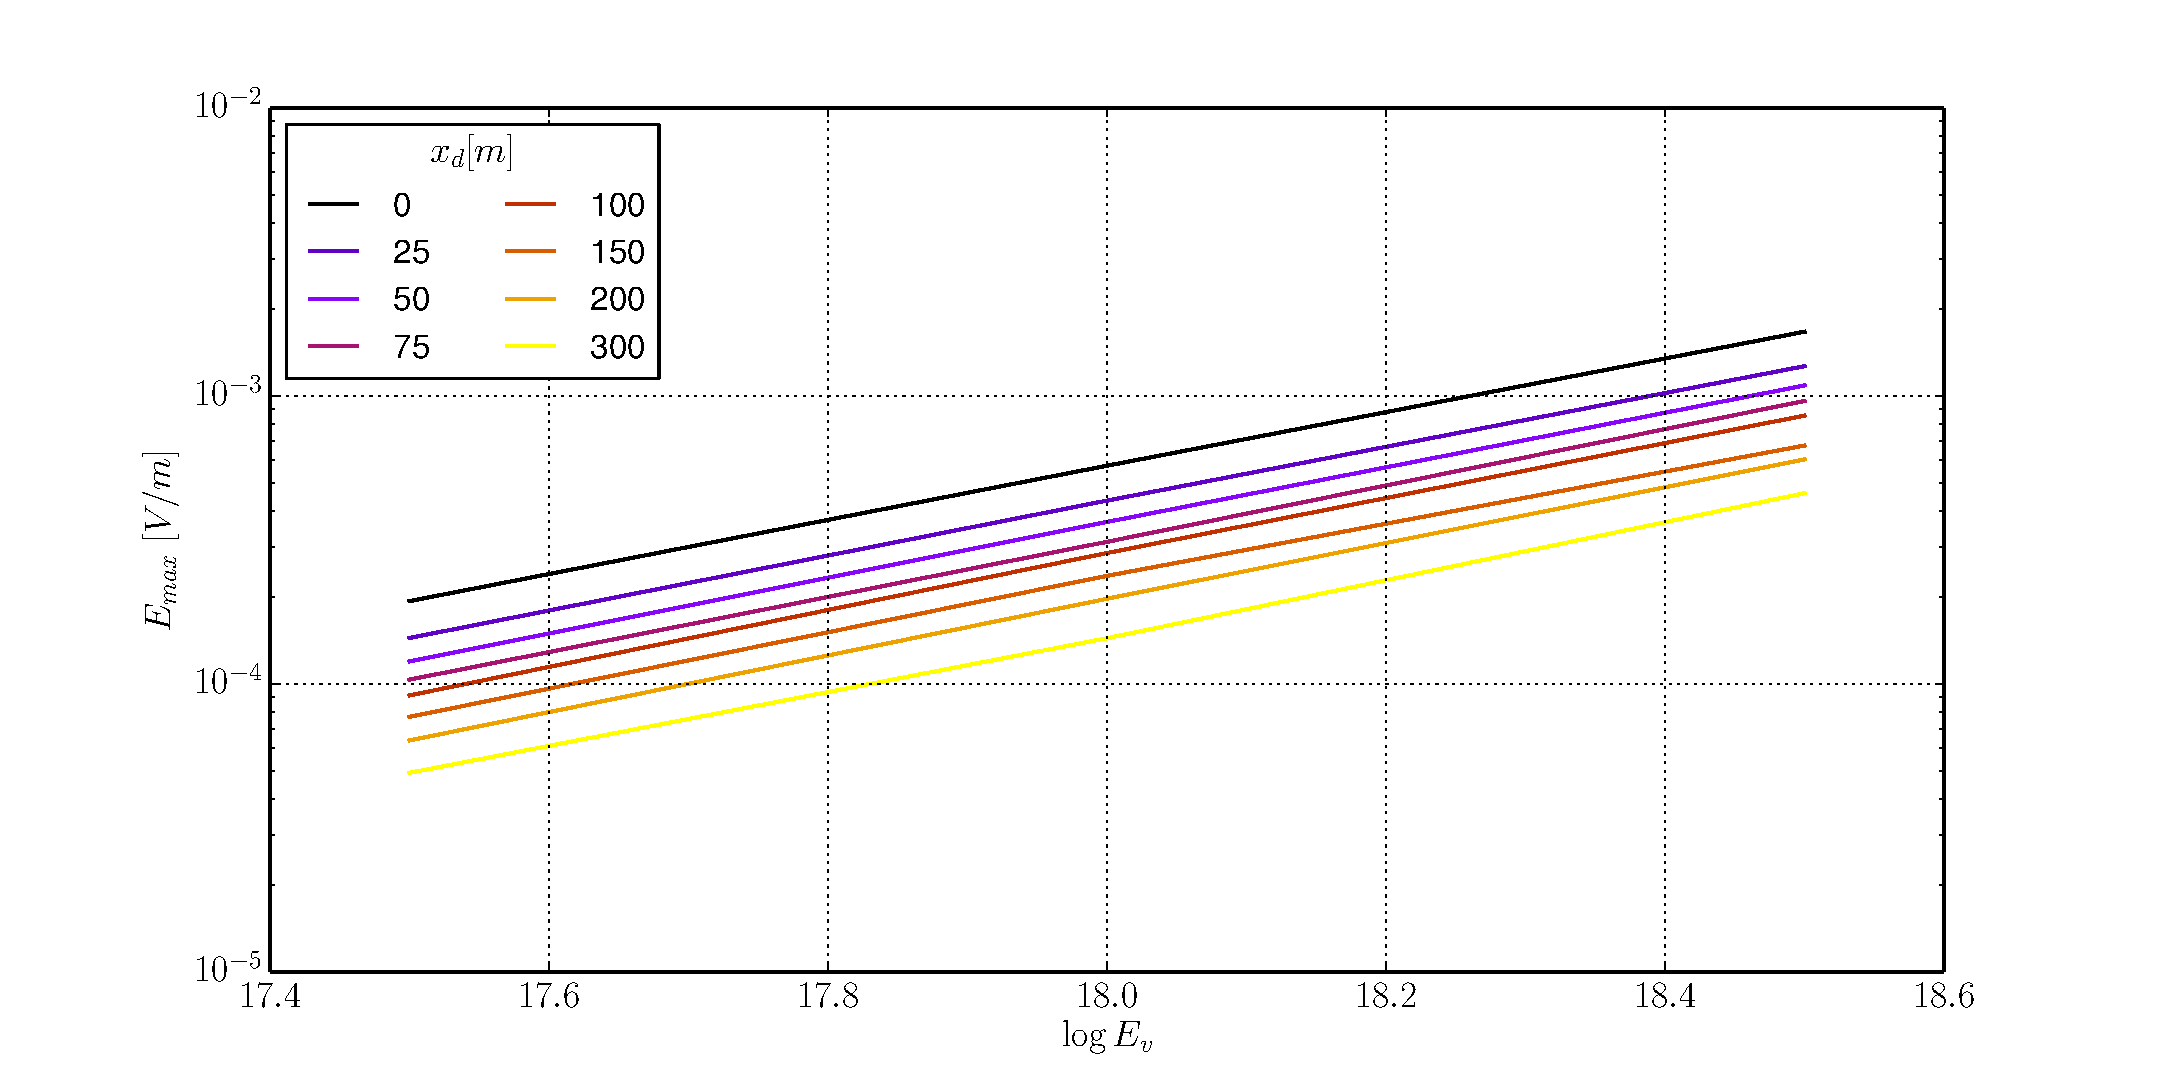
\includegraphics[width=\textwidth]{./fig/simulacionRadio/maxDep/eMaxXdEv}
		\caption{\label{fig:ev_dependence2}
		Arriba (Abajo): M\'aximo campo el\'ectrico registrado en la huella en funci\'on del logaritmo de la energ\'ia visible para varios \'angulos cenitales (varias alturas de decaimiento del \tauon{}).
		Esta cantidad resulta proporcional a la energ\'ia visible en todos los casos.
		}
	\end{figure}
	%
	En todos los casos la dependencia de con la energ\'ia es pr\'acticamente lineal.
	Este comportamiento creciente sugiere, como era natural suponer, que a medida que aumente la energ\'ia visible de la lluvia la eficiencia de detecci\'on crecer\'a.
	
	
	\subsubsection{Dependencia con el canal de decaimiento del \tauon{}}
	\label{sbsc:decayChRadio}
	
	Finalmente es necesario estudiar como afecta el canal de decaimiento del \tauon{} a la huella de radio sobre el detector.
	Dado que el par\'ametro de control de energ\'ia elegido en esta parte de la tesis es la energ\'ia visible, es decir, la que portan las part\'iculas poco penetrantes al inicio de la lluvia, el canal de decaimiento queda determinado por las part\'iculas la inician y por como se distribuye la energ\'ia entre ellas\footnote{Como contraparte, en el an\'alisis para Auger lo que determinaba el decaimiento del \tauon{}, ademas de las part\'iculas y la distribuci\'on de energ\'ia, es qu\'e fracci\'on de la energ\'ia del tau\'on se transmitia a las part\'iculas interactuantes.}.
	Por otro lado, ya se ha expuesto que la emisi\'on de radio en lluvias atmosf\'ericas extendidas depende fuertemente de el n\'umero de part\'iculas de la lluvia, lo que, dada la universalidad de las EAS, se encuentra estrechamente relacionado con la energ\'ia del primario.
	Entonces, a la luz de estos dos hechos se espera que a misma energ\'ia visible y par\'ametros geom\'etricos, el canal de decaimiento del \tauon{} no afecte significativamente las caracter\'isticas de la huella de radio sobre el detector.
	Para poner a prueba esta hip\'otesis, en la figura \ref{fig:tdec_dependence} se muestra la se\~nal a nivel del suelo para cuatro de los canales de decaimiento m\'as representativos. Se observa que las caracter\'isticas generales de la huella se conserva en todos los casos, variando levemente en forma e intensidad.
	%
	\begin{figure}[ht!]
		\centering
		\begin{tabular}{cc}
		$\tau\rightarrow\nu_\tau\pi^-$ - BR=10.9$\%$ & $\tau\rightarrow\nu_\tau\pi^-\pi^-\pi^+$ - BR=9.3$\%$ \\
		\includegraphics[width=0.5\textwidth]{./fig/simulacionRadio/decay/{foorPrint_Cone_ZWv1.22_ntuples_v1.21_ChTest_phi_90_18_89.5_90_25_1005_E0}.png} &
		\includegraphics[width=0.5\textwidth]{./fig/simulacionRadio/decay/{foorPrint_Cone_ZWv1.22_ntuples_v1.21_ChTest_phi_90_18_89.5_90_25_1023_E0}.png}\\
		
		$\tau\rightarrow\nu_\tau e^-\nu_e$ - BR=17.9$\%$ & $\tau\rightarrow\nu_\tau\pi^-\pi^0$ - BR=25.5$\%$ \\
		\includegraphics[width=0.5\textwidth]{./fig/simulacionRadio/decay/{foorPrint_Cone_ZWv1.22_ntuples_v1.21_ChTest_phi_90_18_89.5_90_25_1238_E0}.png} &
		\includegraphics[width=0.5\textwidth]{./fig/simulacionRadio/decay/{foorPrint_Cone_ZWv1.22_ntuples_v1.21_ChTest_phi_90_18_89.5_90_25_1618_E0}.png}\\
		\end{tabular}
		\caption{\label{fig:tdec_dependence}
		Huella de campo el\'ectrico sobre el detector para distintos canales de decaimiento del \tauon{}. Se observa que las caracter\'isticas fundamentales de la misma se mantienen en todos los casos.
		}
	\end{figure}
	%
	
	Por otro lado, para estimar el impacto que podr\'ia llegar a tener el canal de decaimiento  en las eficiencias, la figura \ref{fig:showerVars} muestra las distribuciones del m\'aximo campo el\'ectrico registrado, el \'area sobre la que la se\~nal se mantiene por encima de cierto porcentaje de este m\'aximo ($80\%$ en este caso) y el ancho promedio de la huella.
	%
	\begin{figure}[ht!]
		\centering
		\includegraphics[width=0.7\textwidth]{./fig/simulacionRadio/{showerMaxE_ZWv1.43_ntuples_v1.22_Channels_All}.png}\\
		\includegraphics[width=0.7\textwidth]{./fig/simulacionRadio/{showerArea_ZWv1.43_ntuples_v1.22_Channels_All}.png}\\
		\includegraphics[width=0.7\textwidth]{./fig/simulacionRadio/{showerWidth_ZWv1.43_ntuples_v1.22_Channels_All}.png}
		\caption{\label{fig:showerVars}
		Distribuci\'on de variables de la lluvia relevantes en la detecci\'on, para 50 decaimientos del \tauon{} tomados al azar y para dos alturas de decaimiento diferentes. Arriba: campo el\'ectrico m\'aximo. Medio: \'area cubierta por un campo el\'ectrico que supera el $80\%$ del m\'aximo de la huella. Abajo: ancho promedio de la lluvia. En cada distribuci\'on se detalla la posici\'on del evento de referencia. 
		}
	\end{figure}
	%
	Para construir estas distribuciones se tomaron 30 decaimientos del \tauon{} al azar, respetando los \emph{branching ratios} de la tabla \ref{tab:tauDecay}, y se simul\'o la se\~nal sobre el detector.
	El m\'aximo de la huella se obtuvo simplemente como la m\'axima se\~nal registrada por las antenas simuladas.
	Por otro lado, el \'area sobre el $80\%$ del m\'aximo se determin\'o sumando el \'area representada por cada observador (antena) cuya se\~nal se encontr\'o por sobre este umbral.
	Dado que la distancia entre antenas en la direcci\'on de propagaci\'on es \cant{1}{km} y en la direcci\'on transversal es \cant{100}{m}, cada antena contribuy\'o al \'area total con \cant{0.1}{km^2}.
	Por \'ultimo, el c\'alculo del ancho promedio de la requieri\'o tres pasos.
	Primero se calcul\'o la direcci\'on de propagaci\'on de la se\~nal mediante el ajuste de un frente plano a los tiempos en los que cada antena alcanz\'o su m\'aximo. 
	Segundo, se obtuvo el baricentro de se\~nal de la huella. Tercero, se comput\'o la distancia promedio a la recta determinada por la direcci\'on de propagaci\'on de la se\~nal y por dicho baricentro.
	
	Las variaciones debido al canal de decaimiento observadas en la figura \ref{fig:showerVars} resultan del orden del $10-15\%$ en el m\'aximo campo de la lluvia, de alrededor de $30\%$ en el \'area sobre el umbral y $3\%$ en el ancho promedio.
	Sin embargo, en todos los histogramas se encuentra marcado el bin en el que se ubica el evento de referencia.
	Es interesante notar que su variaci\'on de distribuci\'on a distribuci\'on parece ser menor que la dispersi\'on de cada variable en s\'i, lo que implica correlaci\'on entre ellas.
	Finalmente, tambi\'en se puede notar que el evento de referencia se encuentra en todos los casos cerca del promedio de la distribuci\'on.
	Esto resultar\'a conveniente m\'as adelante, cuando sea necesario determinar el espacio de par\'ametros que se simular\'a para realizar el c\'alculo de exposici\'on.
	
	\textbf{REVSAR}
	
	
\clearpage
\section{Discriminaci\'on en el fondo de eventos hadr\'onicos}
\label{sc:identificacionRadio}

Como se expuso en la primer parte de esta tesis, el mayor desaf\'io a la hora de detectar neutrinos ES mediante detectores de superficie resulta ser su discriminaci\'on en el fondo dominante de eventos hadr\'onicos.
En Auger esto se logra debido a que los tanques \cher{} permiten detectar las lluvias j\'ovenes entre los eventos inclinados, a trav\'es de variables sensibles a la presencia de componente electromagn\'etica.
En un detector de antenas de radio esto no resulta posible debido a que b\'asicamente toda la emisi\'on es generada en el m\'aximo de la lluvia por los electrones de media y baja energ\'ia.
Sin embargo, la geometr\'ia de la emisi\'on permite salvar este escollo, ya que guarda informaci\'on sobre la ubicaci\'on en la que se produjo dicho m\'aximo.
Para representar la situci\'on en la figura \ref{fig:dg_vs_es_radio} se bosqueja el cono \cher{} de un evento DG inclinado, que representa el background, y uno ES.
%
\begin{figure}[ht!]
	\centering
	\includegraphics[width=\textwidth]{./fig/simulacionRadio/idRadio.png}
	\caption{\label{fig:dg_vs_es_radio}
	Esquema de las caracter\'isticas que permiten distinguir los eventos ES del fondo de lluvias hadr\'onicas horizontales (DG). Dado que las lluvias DG se inician alto en la atm\'osfera la apertura del cono \cher{} al nivel de la superficie (l\'inea azul) resulta mucho mayor que la que alcanzar\'ia en un evento ES, debido a que su m\'aximo se produce mucho m\'as cerca de la superficie.
	Adem\'as de la apertura del cono, otro posible factor de discriminaci\'on puede ser la topograf\'ia de la se\~nal a nivel del suelo, ya que en los eventos DG imprimen elipses y los ES hip\'erbolas.
	}
\end{figure}
%
Puede notarse como la apertura del cono del evento DG al nivel de la superficie resulta mayor que el de la se\~nal dejada por el evento ES.
Tambi\'en, se nota como la opograf\'ia de la huella en ambos casos es fundamentalmente distinta, ya que el evento DG imprime una elipse sobre el suelo y el evento ES una hip\'erbola.
En consecuencia se estudiar\'a si es posible explotar estas diferencias para identificar eventos ES.

Por otra parte, en la figura 

- eventos gigantes

- se inician lejos y el campo cae como 1/R pero el drift es mayor debido a la baja densidad de la atm\'osfera

- ver v4.20 en ntuple analizer mostrar que la velocidad sobre el eje y el ancho 


\section{Resumen del an\'alisis de la se\~nal}

\begin{table}[ht!]
\centering
 \begin{tabular}{|p{0.3\textwidth}|p{0.7\textwidth}|}
 \toprule
 Descripci\'on & Detalle \\
 \midrule\midrule
 Filtrado de la se\~nal & Respuesta plana en la banda \cant{30\text{-}80\text{/}120\text{-}900}{MHz} \\ \midrule
 Nivel de disparo local &  Entre \cant{25}{\frac{\mu V}{m}} y \cant{200}{\frac{\mu V}{m}} con un paso de \cant{25}{\frac{\mu V}{m}}\\ \midrule
 Disparo global & Antenas disparadas compatibles con un frente que se desplaza a la velocidad de la luz \\ \midrule
 Nivel de identificaci\'on & Eficiencia entre 0.80 y 1.00 con un paso de 0.05 \\
 
 \bottomrule
 \end{tabular}
\end{table}
